\documentclass{article}
\usepackage[spanish]{babel}
\usepackage{lipsum}
\usepackage{natbib}
\usepackage{graphicx}
\usepackage{analysis_orax}
\usepackage{blindtext}
\usepackage{amsmath}
\usepackage{hyperref}
\usepackage{subcaption} 
\usepackage{float}
\usepackage{listings}
\usepackage{pxfonts}
\usepackage{svg}
\usepackage{pgfplots}
\pgfplotsset{compat=1.11}
\usepackage{enumitem}
\usepackage{tikz}
\usetikzlibrary{shadows}

\newcommand*{\MyShadow}{\tikz \draw [baseline, fill=blue,draw=blue,circular drop shadow] circle (2pt);}
\newcommand*{\MyBall}{\tikz \draw [baseline, ball color=red, draw=red] circle (2pt);}

\definecolor{mGreen}{rgb}{0,0.6,0}
\definecolor{mGray}{rgb}{0.5,0.5,0.5}
\definecolor{mPurple}{rgb}{0.58,0,0.82}
\definecolor{backgroundColour}{rgb}{0.95,0.95,0.92}

\lstdefinestyle{PerlStyle}{
    backgroundcolor=\color{white},   
    commentstyle=\bfseries \color{orange},
    keywordstyle=\color{LightBlue}\bfseries,
    numberstyle=\tiny\color{mPurple},
    stringstyle=\color{red},
    basicstyle=\footnotesize \color{darkgray},
    breakatwhitespace=false,         
    breaklines=true,                 
    captionpos=b,            
    keepspaces=true,                 
    numbers=left,                    
    numbersep=5pt,                  
    showspaces=false,                
    showstringspaces=false,
    showtabs=false,                  
    tabsize=2,
    language=Perl
}


\title{\bigskip \bigskip \bigskip \bigskip \vspace{-15mm}\fontsize{35pt}{35pt}\selectfont\textbf{{Trabajo práctico Nº III - Sistemas Embebidos \\}}
\bigskip \bigskip \fontsize{18pt}{10pt}\selectfont\textbf{\textcolor{teal}{CÁTEDRA DE SISTEMAS OPERATIVOS II}}\bigskip\bigskip \bigskip\bigskip \bigskip}\bigskip\bigskip \bigskip\bigskip \bigskip % Article title
\author{
\large
{
\textsc{Casabella Martin, 39694763 }}\\[2mm]
  martin.casabella@alumnos.unc.edu.ar\\[2mm]
%\thanks{A thank you or further information}\\ % Your name
%\normalsize \href{mailto:marco.torres.810@gmail.com}{marco.torres.810@gmail.com}\\[2mm] % Your email address
\bigskip\bigskip \bigskip \bigskip\bigskip \bigskip
}

\date{\Huge\today}

%------------------Document----------------------------

\begin{document}
\maketitle
\clearpage

%-------------------------TitlePage------------------------
%\begin{titlepage}
%\end{titlepage}
%----------------------------------------------------------------------------------------
%       TITLE SECTION
%----------------------------------------------------------------------------------------

\renewcommand{\figurename}{\textbf{\textcolor{Orange}{Figura}}}
\renewcommand\thefigure{\textbf{\textcolor{Orange}{\arabic{figure}}}}

%-------------------------Content------------------------
\tableofcontents

\clearpage


\section{Introducción}
En la interseccion de Software, Hardware y Comunicaciones nos podemos encontrar a los Sistemas Embebidos. Los mismos son sistemas que, si bien su
definicion varıa con la literatura, se pueden definir como computadoras de uso especıfico, es decir, computadoras con requerimientos de hardware, software y
comunicaciones bien definidos. 
\section{Preparación de entorno}
Como prerrequisito antes de iniciar con el trabajo es necesario la selección de la imagen de linux que utilizaremos en la Raspberry PI 3 Model B (de ahora en adelante rpi),
cómo trabajar con ella. \\

Para la generación de las pruebas trabajamos con la PC local, Arch Linux / Kernel 5.1.5-1 64bits (X86\_64) que tiene distinta configuración del kernel que otras distribuciones
como las basadas en debian.\\
\subsection{Elección del sistema operativo}
Motivos por los cuales se opto por instalar arch:
\begin{itemize}
\item \textbf{Principio KISS:} Nos montamos el sistema como queremos instalando únicamente lo que necesitemos.
\item \textbf{Carácter rolling release:} Nos evitamos la reinstalación de la distribución ya que no se congelan nuevas versiones.
\item \textbf{Gestor de paquetes Pacman:} El gestor de paquetes Pacman es un gestor bastante rápido.
\item \textbf{Yay:} Esta herramienta nos permite usar el repositorio AUR evitando a veces tener que instalar archivos .tar.gz.
\item \textbf{Wiki:} La Wiki de Arch Linux es bastante extensa, pero por contra no está traducida a todos los idiomas
\end{itemize}

Como contras, se tiene que alser rolling release puede causar problemas con algún paquete, aunque Arch Linux es una de las distros más estables, y
la instalación de periféricos como impresoras puede ser tediosa en algunos casos. \\

De todas maneras, en lo que concierne a este trabajo practico se opto principalmente porque es un linux extremadamente liviano por tener la filosofía
Arch Way, mejor resumido por el acrónimo KISS. \\

\subsection{Configuración Raspberry}

En el servidor (Raspberry Pi 3 Model B), luego de instalar el Sistema Operativo, se instalaron las siguientes herramientas:\\

\begin{lstlisting}[style=PerlStyle]
pacman -Syu  # update sistema
pacman -S --needed base-devel #herramientas basicas de utilidad
pacman -S vim git p7zip nmap nload community/mc
pacman -S wget community/sysstat 
pacman -S community/perl-cgi #modulo cgi de PERL
pacman -S community/aws-cli #AWS


vim /etc/ssh/sshd_config  #cfg ssh


systemctrl enable sshd # Restauramos el servicio 
systemctrl restart sshd # nos aseguramos que este corriendo

\end{lstlisting}

A su vez, los siguientes modulos de Perl son necesarios:
\begin{lstlisting}[style=PerlStyle]
sudo cpanm Linux::SysInfo #info sistema
sudo cpanm Linux::Cpuinfo #info procesador
sudo cpanm File::basename #manejo de archivos
\end{lstlisting}

\section{Elección WebServer}

Se tomaron en cuenta las opciones más estables, seguras y de mejor rendimiento: apache, nginx y lighttpd. \\

Se prioriza un servidor liviano ya que va a correr en el embebido simplemente para esta aplicación. Ademas, se prioriza que \textit{no tenga características que no serán utilizadas} (como Apache), y Lighttpd fue electo. \\

Lighttpd es un software escrito en C por Jan Kneschke, se distribuye bajo la licencia BSD y está disponible para Unix y Linux. na de las características del servidor web es que consume realmente pocos recursos a nivel de RAM y CPU, haciéndolo especialmente útil para VPS o Dedicados de bajos recursos, además de que es ideal para balancear cargas por RRDNS.\\

Soporta comunicación e integración con FastCGI, SCGI y CGI, por lo que es capaz de servir requests de páginas hechas en cualquier lenguaje de programación.\\

\subsection{Nginx - Apache - Lighttpd}
\begin{figure}[H]
    \centering
      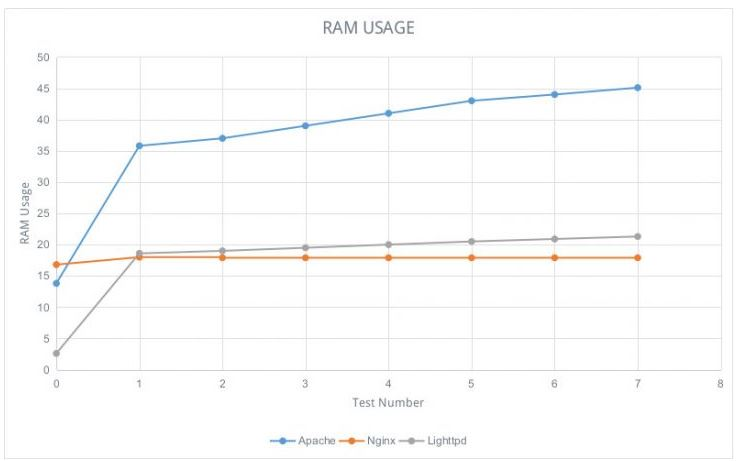
\includegraphics[width=0.68\textwidth]{figures/r1.jpg}
       \centering
       \caption{\textbf{\textcolor{Orange}{Uso de memoria}}}       
    \end{figure}

\begin{figure}[H]
    \centering
      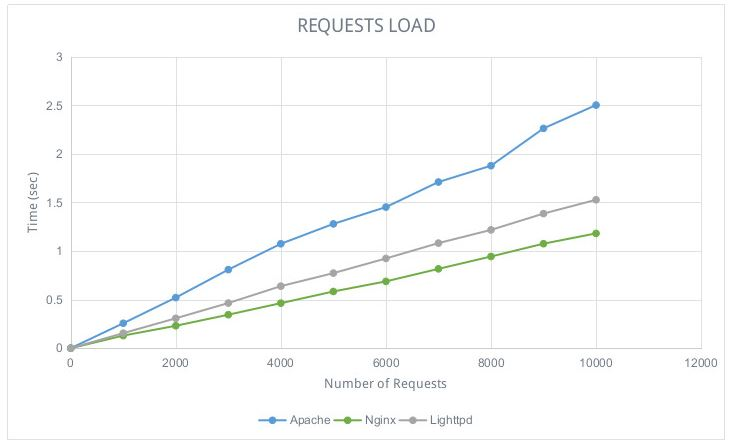
\includegraphics[width=0.8\textwidth]{figures/r2.jpg}
       \centering
       \caption{\textbf{\textcolor{Orange}{Respuesta a solicitudes (performance)}}}       
    \end{figure}

\begin{figure}[H]
    \centering
      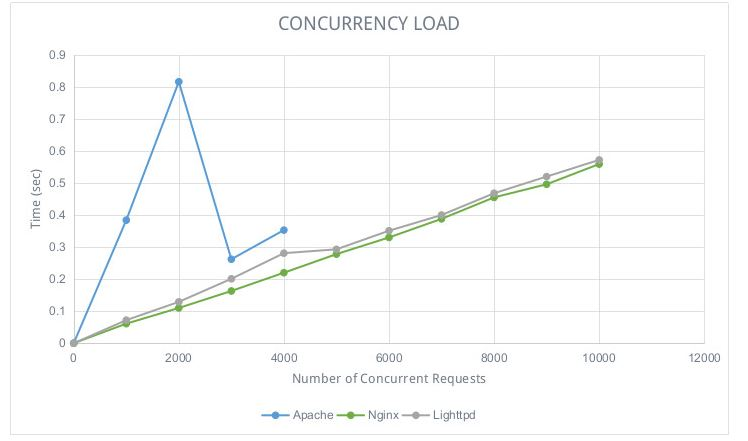
\includegraphics[width=0.8\textwidth]{figures/r3.jpg}
       \centering
       \caption{\textbf{\textcolor{Orange}{Concurrencia (performance)}}}       
    \end{figure}


\subsection{Fast CGI}
FastCGI es un protocolo para interconectar programas interactivos con un servidor web, donde se modifica Common Gateway Interface (CGI ó Interfaz Común de Entrada).\\

El principal objetivo de FastCGI es reducir la carga asociada con el hecho de interconectar el servidor web y los programas Common Gateway Interface, permitiéndole a un servidor atender más peticiones a la vez.\\

En vez de crear procesos nuevos por cada petición, FastCGI puede usar un solo proceso persistente que maneja cualquier petición durante su período de vida. El hecho de procesar múltiples peticiones a la vez es logrado ya sea mediante la utilización de una sola conexión con un multiplexado interno (por ejemplo múltiples peticiones sobre una sola conexión) y/o utilizando múltiples conexiones. \\

 FastCGI proporciona alto rendimiento y persistencia sin las limitaciones de las API específicas del servidor.Varios de esos procesos pueden existir, y eso es algo que incrementa la escalabilidad y el rendimiento. FastCGI permite también a los programas hacer que el servidor web realice ciertas operaciones sencillas, como leer un archivo antes de que la petición sea procesada.\\

La mencion de Fast CGI recae en el porque descartar opciones como \textbf{Nginx} , que no soporta CGI, sino que utiliza Fast CGI. \\

\section{Sintesis: diferencias}
\begin{itemize}

\item Tanto Apache como Lighttpd poseen actualmente inconvenientes como pérdidas de memoria

\item Apache es el único servidor de los tres que ofrece una anulación de acceso a todo el sistema, lo que quizás sea una característica insustituible para los servicios de alojamiento compartido.

\item Teniendo en cuenta los tres aspectos principales de un servidor web: características, uso de memoria y rendimiento, parece que Nginx llegó a la cima por ahora.

\item Lighttpd funciona como un proceso único, mientras que Nginx funciona como un proceso maestro.

\item  En un sistema de archivos fragmentado funciona mejor en comparación con Nginx Lighttpd.

\item La CPU utilizada por Nginx es mucho menos Lighttpd.

\item Lighttpd admite IPv6 mientras se procesa la compatibilidad con Nginx IPv6.

\item  La función de registro de errores independiente es compatible con Nginx pero no es compatible con Lighttpd.

\item Mientras que el servicio de archivos estáticos con un único servidor HTTP Lighttpd proporciona una configuración simple, pero Nginx es más difícil en el caso.

\item US Lighttpd fue popular Nginx. Full Bug Tracking System es compatible con Lighttpd en Nginx tiene el sistema de seguimiento de errores de un hombre pobre.

\item	Los canales IRC son compatibles con Lighttpd como Nginx, pero los canales Nginx son muy silenciosos y tienen grandes retrasos para responder las preguntas de los usuarios.
\end{itemize}

Se opto por Lighttpd dado el contexo, el sistema operativo instalado, características de la aplicación (requerimientos) y uso de recursos. \\




\subsection{Instalación Lighttpd}
\begin{lstlisting}[style=PerlStyle]
pacman -S extra/lighttpd  #instalamos el sv
systemctl enable lighttpd  #lo habilitamos
vim /etc/lighttpd/lighttpd.conf # Editamos la configuración del server para modulos CGI
systemctl status lighttpd  #lo largamos a correr
systemctl start lighttpd
systemctl status lighttpd
\end{lstlisting}


\section{Perl scripting y HTML: How-to}

Para CGI utilizamos todo por Perl Scripting debido a potencia en la manipulación de cadenas de texto, los diferentes script y la instalación de los módulos se detallan a
continuación.\\

Por su parte, se combino el desarrollo con HTML (HyperText Markup Language) por simplicidad. El usuario opta por clickear una pestaña u otra según lo que desee, y al realizar
las acciones posibles (listar módulos, listar aws, subir modulo de kernel e instalarlo, obtener información del sistema) se llama a un script hecho en Perl, que se encarga de ejecutar los 
comandos necesarios segun lo solicitado.\\
\subsection{Home}
La pagina principal permite al usuario elegir una pestaña u otra según lo que desee hacer.\\ 
Según su elección, se referencia a distintos archivos, encargados de obtener el resultado buscado.
\subsubsection{index.html}
\lstinputlisting[    language=HTML,
     basicstyle=\scriptsize, %or \small or \footnotesize etc.
	     identifierstyle=\color{magenta},
	      keywordstyle=\color{cyan}\bfseries,
	       commentstyle=\bfseries \color{darkgray},
     stringstyle=\color{blue}
   ]{index.html}
   

El script referencia diferentes scripts que se ejecutan según la pestaña correspondiente.\\

\subsection{System Resources}
Simplemente referencia un script en perl, encargado de ejecutarse y obtener informacion deseada del sistema segun los requerimientos. Para ello se utilizan módulos
disponibles en Perl, como Linux::SysInfo, y Linux::CpuInfo, que hacen de interfaz con las llamadas del sistema operativo.\\
\subsubsection{system\_info.pl}
\begin{lstlisting}[style=PerlStyle]
#!/usr/bin/perl
use strict;
use warnings FATAL => 'all';
use lib qw<blib/lib blib/arch>;

use CGI::Carp qw(fatalsToBrowser);
use Linux::SysInfo qw<sysinfo>;
use Proc::CPUUsage;
use Unix::Uptime qw(:hires);


#para uso CPU
my $cp = Proc::CPUUsage->new;
#para sys info
my $si = sysinfo;

my @months = qw( Jan Feb Mar Apr May Jun Jul Aug Sep Oct Nov Dec );
my @days = qw(Sun Mon Tue Wed Thu Fri Sat Sun);
my ($sec,$min,$hour,$mday,$mon,$year,$wday,$yday,$isdst) = localtime();
$year += 1900;

#Date/time
my $current_date = "$days[$wday] $mday $months[$mon] $year";
my $current_time = "$hour:$min:$sec";

#CPU usage
my $usage1 = $cp->usage*100; ## returns usage since new()
my $usage2 = $cp->usage*100; ## returns usage since last usage()

#Uptime
my $uptime = Unix::Uptime->uptime(); # 2345
# # "HiRes" mode
my $uptime_sec =Unix::Uptime->uptime_hires();

my ($load1, $load5, $load15) = Unix::Uptime->load(); # (1.0, 2.0, 0.0)



#HTML FORMAT PAGE
print "Content-type: text/html\n\n";

print "<html>\n";
print "<head>";
print "<title>Sistemas Operativos II</title>";
print "<meta name=\"description\" content=\"website description\" /> ";
print "<meta name=\"keywords\" content=\"website keywords, website keywords\" />";
print "<meta http-equiv=\"content-type\" content=\"text/html; charset=windows-1252\" />";
print "<link rel=\"stylesheet\" type=\"text/css\" href=\"http://fonts.googleapis.com/css?family=Tangerine&amp;v1\" />";
print "<link rel=\"stylesheet\" type=\"text/css\" href=\"http://fonts.googleapis.com/css?family=Yanone+Kaffeesatz\"/>";
print "<link rel=\"stylesheet\" type=\"text/css\" href=\"../style/style.css\" />";
print "</head>";


print "<body>";
<body bgcolor="#ff69b4" value="F" >;
print "<div id=\"main\">";
print "<div id=\"header\">";
print "<div id=\"logo\">";
print "<h1>Sistemas Operativos II</h1>";
print "</div>";
print "<div id=\"menubar\">";
print "<ul id=\"menu\">";
print "<li><a href=\"../index.html\">Home</a></li>";
print "<li class=\"current\"><a href=\"system_info.pl\">System Resources</a></li>";
print "<li><a href=\"../goes.html\">GOES Info</a></li>";
print "<li><a href=\"modules.pl\">System modules</a></li>";
print "<li><a href=\"../upload_module.html\">Install module</a></li>";
print "</ul>";
print "</div>";
print "</div>";


print "<div id=\"content\">";
print "<h1>System Resources</h1>";
print "<p>Date: $current_date        Time: $current_time";
print "<p><p>System information:</p>";
print "<p>- $_: $si->{$_}" for keys %$si;
print "<p>- CPU usage (last measurement):  $usage2 %</p>";
print "<p> -Uptime: " , $uptime_sec, " [s]</p>";
print "<p> -Load average for last minute: " ,$load1, </p>;

print "     <p></p>";
print "  <p></p>";
print "      <p></p>";
print "   <p></p>";

print "</div>";
print "</div>";
print "<p></p>";
print "<p></p>";

print " <div id=\"footer\">";
print "Martin Casabella</p>martin.casabella\@alumnos.unc.edu.ar</p>";
print " </div>";
print " </div>";
print " </body>";
print "  </html>";

\end{lstlisting}
\subsection{GOES Info}
Devuelta, al elegir esta pestana, se referencia primero a un archivo html, que mediante un formulario que se le brinda al usuario, obtiene la fecha deseada  mediante un formulario
y que al enviarlo, devuelve la lista del archivos disponibles de Goes 16 en AWS (producto ABI-L2-CMIPF, canal 13) y  los muestra en la pagina. Para ello, desde este archivo
se ejecuta un nuevo script hecho en Perl, que parsea este ingreso, y ejecuta el comando aws para obtener la información deseada.\\

\subsubsection{goes.html}
\lstinputlisting[    language=HTML,
     basicstyle=\scriptsize, %or \small or \footnotesize etc.
	     identifierstyle=\color{magenta},
	      keywordstyle=\color{cyan}\bfseries,
	       commentstyle=\bfseries \color{darkgray},
     stringstyle=\color{blue}
   ]{goes.html}
   

\subsubsection{aws.pl}
\begin{lstlisting}[style=PerlStyle]
#!/usr/bin/perl -w
use warnings;
use strict;
use CGI qw(:standard);
use CGI::Carp qw(fatalsToBrowser);
use File::Basename;
use File::chdir;
#Instancia CGI
my $query = new CGI;


#obtengo fecha como parametro del ususario
my $date = $query->param("date");
#my $date = "2019/025/01";
my @words = split '/', $date;

my $year = $words[0];
my $day = sprintf '%03s', $words[1];
my $hour = sprintf '%02s', $words[2];


#Ejecuto comando aws, y parseo su salida, para asi imprimirla
my $raw_out  = qx(/usr/bin/aws --no-sign-request s3 ls s3://noaa-goes16/ABI-L2-CMIPF/$year/$day/$hour/ 2>&1);

#print `/usr/bin/aws --no-sign-request s3 ls s3://noaa-goes16/ABI-L2-CMIPF/2019/001/23/ 2>&1`;
my @lines = split /\n/, $raw_out;


#Muestro pagina html para seguir formato de las demas
print "Content-type: text/html\n\n";

print "<html>\n";
print "<head>";
print "<title>Sistemas Operativos II</title>";
print "<meta name=\"description\" content=\"website description\" /> ";
print "<meta name=\"keywords\" content=\"website keywords, website keywords\" />";
print "<meta http-equiv=\"content-type\" content=\"text/html; charset=windows-1252\" />";
print "<link rel=\"stylesheet\" type=\"text/css\" href=\"http://fonts.googleapis.com/css?family=Tangerine&amp;v1\" />";
print "<link rel=\"stylesheet\" type=\"text/css\" href=\"http://fonts.googleapis.com/css?family=Yanone+Kaffeesatz\"/>";
print "<link rel=\"stylesheet\" type=\"text/css\" href=\"../style/style.css\" />";
print "</head>";


print "<body>";
<body bgcolor="#ff69b4" value="F" >;
print "<div id=\"main\">";
print "<div id=\"header\">";
print "<div id=\"logo\">";
print "<h1>Sistemas Operativos II</h1>";
print "</div>";
print "<div id=\"menubar\">";
print "<ul id=\"menu\">";
print "<li><a href=\"../index.html\">Home</a></li>";
print "<li ><a href=\"system_info.pl\">System Resources</a></li>";
print "<li class=\"current\" ><a href=\"../goes.html\">GOES Info</a></li>";
print "<li><a href=\"modules.pl\">System modules</a></li>";
print "<li><a href=\"../upload_module.html\">Install module</a></li>";
print "</ul>";
print "</div>";
print "</div>";


print "<div id=\"content\">";
print "<h1>GOES 16 archives</h1>";

print "$year\n";
print "$day\n";
print "$hour\n";
print"<p><\p>";

# Imprimo lista de archivos en el html para que el usuario vea lo solicitado
foreach my $line (@lines) {
    my @entry = split('\s+',$line,4);
    print "$entry[0]      $entry[1]   $entry[2]       $entry[3] ";


}

print "      <p></p>";
print "   <p></p>";
print "      <p></p>";
print "    <p></p>";
print "        <p></p>";

print "</div>";
print "</div>";
print "<p></p>";
print "<p></p>";

print " <div id=\"footer\">";
print "Martin Casabella</p>martin.casabella\@alumnos.unc.edu.ar</p>";
print " </div>";
print " </div>";
print " </body>";
print "  </html>";
\end{lstlisting}


\subsection{System Modules}
Aqui se satisface el requerimiento de devolver en la pagina la lista con modulos instalados. Para ello, se utiliza el comando $lnsmod$.  Una prueba que se realizo es probar obtener la lista, proceder a instalar el 
modulo (con la otra pestana) y volver a pedir la lista, verificando que se haya instalado el modulo. \\
\bigskip
\subsubsection{module.pl}
\begin{lstlisting}[style=PerlStyle]
#!/usr/bin/perl
use strict;
use warnings FATAL => 'all';
use lib qw<blib/lib blib/arch>;
use CGI qw(:standard);


#Obtengo lista de modulos
my $out = qx(lsmod 2>&1);
#my @lines = split /\n/, $out; #guardo en array lines, lista partida en \n


print "Content-type: text/html\n\n";

print "<html>\n";
print "<head>";
print "<title>Sistemas Operativos II</title>";
print "<meta name=\"description\" content=\"website description\" /> ";
print "<meta name=\"keywords\" content=\"website keywords, website keywords\" />";
print "<meta http-equiv=\"content-type\" content=\"text/html; charset=windows-1252\" />";
print "<link rel=\"stylesheet\" type=\"text/css\" href=\"http://fonts.googleapis.com/css?family=Tangerine&amp;v1\" />";
print "<link rel=\"stylesheet\" type=\"text/css\" href=\"http://fonts.googleapis.com/css?family=Yanone+Kaffeesatz\"/>";
print "<link rel=\"stylesheet\" type=\"text/css\" href=\"../style/style.css\" />";
print "</head>";

print "<body>";
<body bgcolor="#ff69b4" value="F" >;
print "<div id=\"main\">";
print "<div id=\"header\">";
print "<div id=\"logo\">";
print "<h1>Sistemas Operativos II</h1>";
print "</div>";
print "<div id=\"menubar\">";
print "<ul id=\"menu\">";
;

print "<li><a href=\"../index.html\">Home</a></li>";
print "<li><a href=\"system_info.pl\">System Resources</a></li>";
print "<li><a href=\"../goes.html\">GOES Info</a></li>";
print "<li class=\"current\"><a href=\"modules.pl\">System modules</a></li>";
print "<li><a href=\"../upload_module.html\">Install module</a></li>";
print "</ul>";
print "</div>";
print "</div>";

print "<div id=\"content\">";
print "<h1>Installed system modules</h1>";


#Parseo salida lsmod y la muestro en pantalla
my @lines = split /\n/, $out;

#Ssimplemente para obviar la primera linea de salida
my $first = 1;
foreach my $line (@lines) {
    my @entry = split('\s+',$line,3);

    if ($first==1){
        $first = 0;
    }else{
        print "<p> Module:   $entry[0]  &nbsp;  Size:   $entry[1]  &nbsp; Used by:   $entry[2] ";
    }
}


print "</div>";
print "</div>";
print "<p></p>";
print "<p></p>";

print " <div id=\"footer\">";
print "Martin Casabella</p>martin.casabella\@alumnos.unc.edu.ar</p>";
print " </div>";
print " </div>";
print " </body>";
print "  </html>";


\end{lstlisting}
\subsection{Install module}
Se tienen dos instancias para proceder a instalar un modulo: verificar que el archivo sea valido, y luego enviarlo para instalarlo. Todo se realizo en otro script en Perl, donde se valida primero el archivo verificando extension .ko, y luego
se envia hacia el servidor, donde se coloca en el directorio definido para las cargas $uploads$. \\
Una vez validado y enviado, desde el mismo script, se ejecuta el comando $insmod module.ko$ para proceder a cargarlo. Se handlean diferentes errores en el script (mala extension, no existencia del archivo, entre otros).\\

\subsubsection{upload\_module.html}
\lstinputlisting[    language=HTML,
     basicstyle=\scriptsize, %or \small or \footnotesize etc.
	     identifierstyle=\color{magenta},
	      keywordstyle=\color{cyan}\bfseries,
	       commentstyle=\bfseries \color{darkgray},
     stringstyle=\color{blue}
   ]{upload_module.html}
   
   \bigskip
   
\subsubsection{upload\_module.pl}
\begin{lstlisting}[style=PerlStyle]
#!/usr/bin/perl
use strict;
use warnings FATAL => 'all';
use CGI;
use CGI::Carp qw ( fatalsToBrowser );
use File::Basename;
use File::chdir;




print "Content-type: text/html\n\n";

print "<html>\n";
print "<head>";
print "<title>Sistemas Operativos II</title>";
print "<meta name=\"description\" content=\"website description\" /> ";
print "<meta name=\"keywords\" content=\"website keywords, website keywords\" />";
print "<meta http-equiv=\"content-type\" content=\"text/html; charset=windows-1252\" />";
print "<link rel=\"stylesheet\" type=\"text/css\" href=\"http://fonts.googleapis.com/css?family=Tangerine&amp;v1\" />";
print "<link rel=\"stylesheet\" type=\"text/css\" href=\"http://fonts.googleapis.com/css?family=Yanone+Kaffeesatz\"/>";
print "<link rel=\"stylesheet\" type=\"text/css\" href=\"../style/style.css\" />";
print "</head>";


print "<body>";
<body bgcolor="#ff69b4" value="F" >;
print "<div id=\"main\">";
print "<div id=\"header\">";
print "<div id=\"logo\">";
print "<h1>Sistemas Operativos II</h1>";
print "</div>";
print "<div id=\"menubar\">";
print "<ul id=\"menu\">";
print "<li><a href=\"../index.html\">Home</a></li>";
print "<li ><a href=\"system_info.pl\">System Resources</a></li>";
print "<li><a href=\"../goes.html\">GOES Info</a></li>";
print "<li><a href=\"modules.pl\">System modules</a></li>";
print "<li class=\"current\" ><a href=\"../upload_module.html\">Install module</a></li>";
print "</ul>";
print "</div>";
print "</div>";


print "<div id=\"content\">";
print "<h1>Install or remove kernel module</h1>";



$CGI::POST_MAX = 1024 * 5000;

# my $safe_filename_characters = "a-zA-Z0-9_.-";
my $upload_dir = "/srv/http/uploads";
my $query = new CGI;
my $filename = $query->param("module");

#COn el parametro module recibido (y archivo) procedo a validarlo

if ( !$filename ) {
    # print $query->header ( );
    # print "There was a problem uploading your photo (try a smaller file).";
    print "<p>Iput not interpreted\n\n";
    exit;
}


#Parseo la extension
my ( $name, $path, $extension ) = fileparse ( $filename, '..*' );
$filename = $name . $extension;

$filename =~ tr/ /_/;
# $filename =~ s/[^$safe_filename_characters]//g;

if ($filename =~ /^(\w+[\w.-]+\.ko)$/o) {
    $filename = $1;
    print "<p> Checked file: [ OK ]. <p>"
}
else {
    die "<p> Not a module file<p>";
}

my $upload_filehandle = $query->upload("module");

open ( UPLOADFILE, ">$upload_dir/$filename" ) or die "$!";
binmode UPLOADFILE;

while ( <$upload_filehandle> ){
    print UPLOADFILE;
}

close UPLOADFILE;


chdir "../uploads";
print `/usr/bin/sudo /usr/bin/insmod $filename`;
print " Module uploaded to server and installed correctly <p>.";

print "      <p></p>";
print "   <p></p>";
print "      <p></p>";
print "    <p></p>";
print "        <p></p>";

print "</div>";
print "</div>";
print "<p></p>";
print "<p></p>";

print " <div id=\"footer\">";
print "Martin Casabella</p>martin.casabella\@alumnos.unc.edu.ar</p>";
print " </div>";
print " </div>";
print " </body>";
print "  </html>";

\end{lstlisting}

\bigskip


\subsubsection{rm\_module.pl}

Da como supuesto que el modulo a remover, es uno previamente cargado por el usuario, por lo que debe existir como requisito, el archivo $module.ko$ en la carpeta uploads. \\

Si este no existe en la misma, no se efectua ninguna operacion, ya que puede recaer en la descarga de algun modulo existente en el servidor. Si existe, se ejecuta $rmmod module.ko$ y luego se borra el archivo $.ko$ del directorio uploads. Nuevamente, se realizo todo en Perl.\\


\begin{lstlisting}[style=PerlStyle]
#!/usr/bin/perl
use strict;
use warnings FATAL => 'all';
use CGI;
use CGI::Carp qw ( fatalsToBrowser );
use File::Basename;
use File::chdir;




print "Content-type: text/html\n\n";

print "<html>\n";
print "<head>";
print "<title>Sistemas Operativos II</title>";
print "<meta name=\"description\" content=\"website description\" /> ";
print "<meta name=\"keywords\" content=\"website keywords, website keywords\" />";
print "<meta http-equiv=\"content-type\" content=\"text/html; charset=windows-1252\" />";
print "<link rel=\"stylesheet\" type=\"text/css\" href=\"http://fonts.googleapis.com/css?family=Tangerine&amp;v1\" />";
print "<link rel=\"stylesheet\" type=\"text/css\" href=\"http://fonts.googleapis.com/css?family=Yanone+Kaffeesatz\"/>";
print "<link rel=\"stylesheet\" type=\"text/css\" href=\"../style/style.css\" />";
print "</head>";


print "<body>";
<body bgcolor="#ff69b4" value="F" >;
print "<div id=\"main\">";
print "<div id=\"header\">";
print "<div id=\"logo\">";
print "<h1>Sistemas Operativos II</h1>";
print "</div>";
print "<div id=\"menubar\">";
print "<ul id=\"menu\">";
print "<li><a href=\"../index.html\">Home</a></li>";
print "<li ><a href=\"system_info.pl\">System Resources</a></li>";
print "<li><a href=\"../goes.html\">GOES Info</a></li>";
print "<li><a href=\"modules.pl\">System modules</a></li>";
print "<li class=\"current\" ><a href=\"../upload_module.html\">Install module</a></li>";
print "</ul>";
print "</div>";
print "</div>";


print "<div id=\"content\">";
print "<h1>Install or remove kernel module</h1>";
print "<p> Module removed <p>";
#Cambio a directorio de carga del sv
chdir "../uploads";
#Defino path
my $dirname = "/srv/http/uploads";
#abro directorio y handlero error
opendir ( DIR, $dirname ) || die "Error in opening dir $dirname\n";
#busco .ko files, para removerlas
my @files = grep(/\.ko$/,readdir(DIR));
closedir(DIR);
#Si hay alguna, significa que el ususario previamente envio el modulo (lo cargo e instalo).
#Lo remuevo, y borro el .ko del directorio del sv
foreach my $file (@files) {
      print `/usr/bin/sudo /usr/bin/rmmod $file`;
      print `/usr/bin/sudo /usr/bin/rm $file`;
}




print "      <p></p>";
print "   <p></p>";
print "      <p></p>";
print "    <p></p>";
print "        <p></p>";

print "</div>";
print "</div>";
print "<p></p>";
print "<p></p>";

print " <div id=\"footer\">";
print "Martin Casabella</p>martin.casabella\@alumnos.unc.edu.ar</p>";
print " </div>";
print " </div>";
print " </body>";
print "  </html>";

\end{lstlisting}


\section{POST, GET y CGI}

Introduciendo, se sabe que GET se utiliza para solicitar datos de un recurso específico, mientras que POST se utiliza para enviar datos a un servidor para crear / actualizar un recurso.\\

Referenciando CGI,La principal diferencia entre estos métodos es la forma en que los datos del formulario se pasan al programa CGI. \\

\begin{itemize}
\item Si se utiliza el método GET, la cadena de consulta simplemente se agrega a la URL del programa cuando el cliente envía la solicitud al servidor. Se puede acceder a esta cadena de consulta utilizando la variable de entorno QUERY\_STRING. 
\item Para obtener datos enviados por el método POST, el programa CGI lee desde $stdin$
\end{itemize}

El servidor necesita una forma de saber qué URL se asignan a los scripts y qué URL solo se asignan a los archivos HTML normales. Para CGI, esto suele hacerse mediante la creación de directorios CGI en el servidor.\\

Esto se hace en la configuración del servidor y le dice al servidor que todos los archivos en un directorio de nivel superior en particular son scripts CGI (ubicados en algún lugar del disco) que se ejecutarán cuando se solicite. (El directorio predeterminado suele ser / cgi-bin /, por lo que se puede decir que las URL así: http://www.varsity.edu/cgi-bin/search apuntan a una secuencia de comandos CGI. Tenga en cuenta que el directorio puede llamarse de cualquier manera .)\\

Básicamente, CGI funciona así: se envía una URL al servidor, que usa CGI para ejecutar un programa. El servidor pasa la entrada al programa y la salida del programa de vuelta al emisor.  CGI actúa como una "puerta de enlace" entre el servidor y el programa escrito.\\

El principio básico de Common Gateway Interface (CGI) es que un servidor web pasa la información de solicitud del cliente a los programas CGI en las variables de entorno del sistema (y en algunos casos a través de argumentos de línea de comando o entrada estándar) y toda la salida estándar de los programas CGI se devuelve a la Web (clientela).\\

Cuando las variables de entorno han sido establecidas por el servidor HTTP, inicia el programa CGI. Depende de este programa CGI averiguar dónde obtener la información necesaria para cumplir con la solicitud.\\


\subsection{CGI: procesando entradas}
Cuando las variables de entorno han sido establecidas por el servidor HTTP, inicia el programa CGI. (Para obtener una lista completa de las variables de entorno establecidas por el servidor HTTP, consulte las variables de entorno establecidas por el servidor HTTP). Luego, depende de este programa CGI averiguar dónde obtener la información necesaria para cumplir con la solicitud.\\

\subsection{Procesando solicitud}
Procesar la solicitud es la segunda etapa de un programa CGI. En esta etapa, el programa toma los datos analizados y realiza la acción apropiada

\subsection{Respuesta}
Cuando el programa CGI ha terminado de procesarse, debe enviar su resultado al servidor HTTP que invocó el programa. Al hacerlo, la salida se envía indirectamente al cliente que inicialmente solicitó la información.\\

Debido a que el programa CGI emite su resultado a través de STDOUT, el servidor HTTP debe leer la información desde allí e interpretar qué hacer.\\

Un programa CGI escribe un encabezado CGI que es seguido por un cuerpo de entidad en la salida estándar. El encabezado CGI es la información que describe los datos en el cuerpo de la entidad. El cuerpo de la entidad son los datos que el servidor envía al cliente.\\

\section{Implementacion y resultados}
\begin{figure}[H]
    \centering
      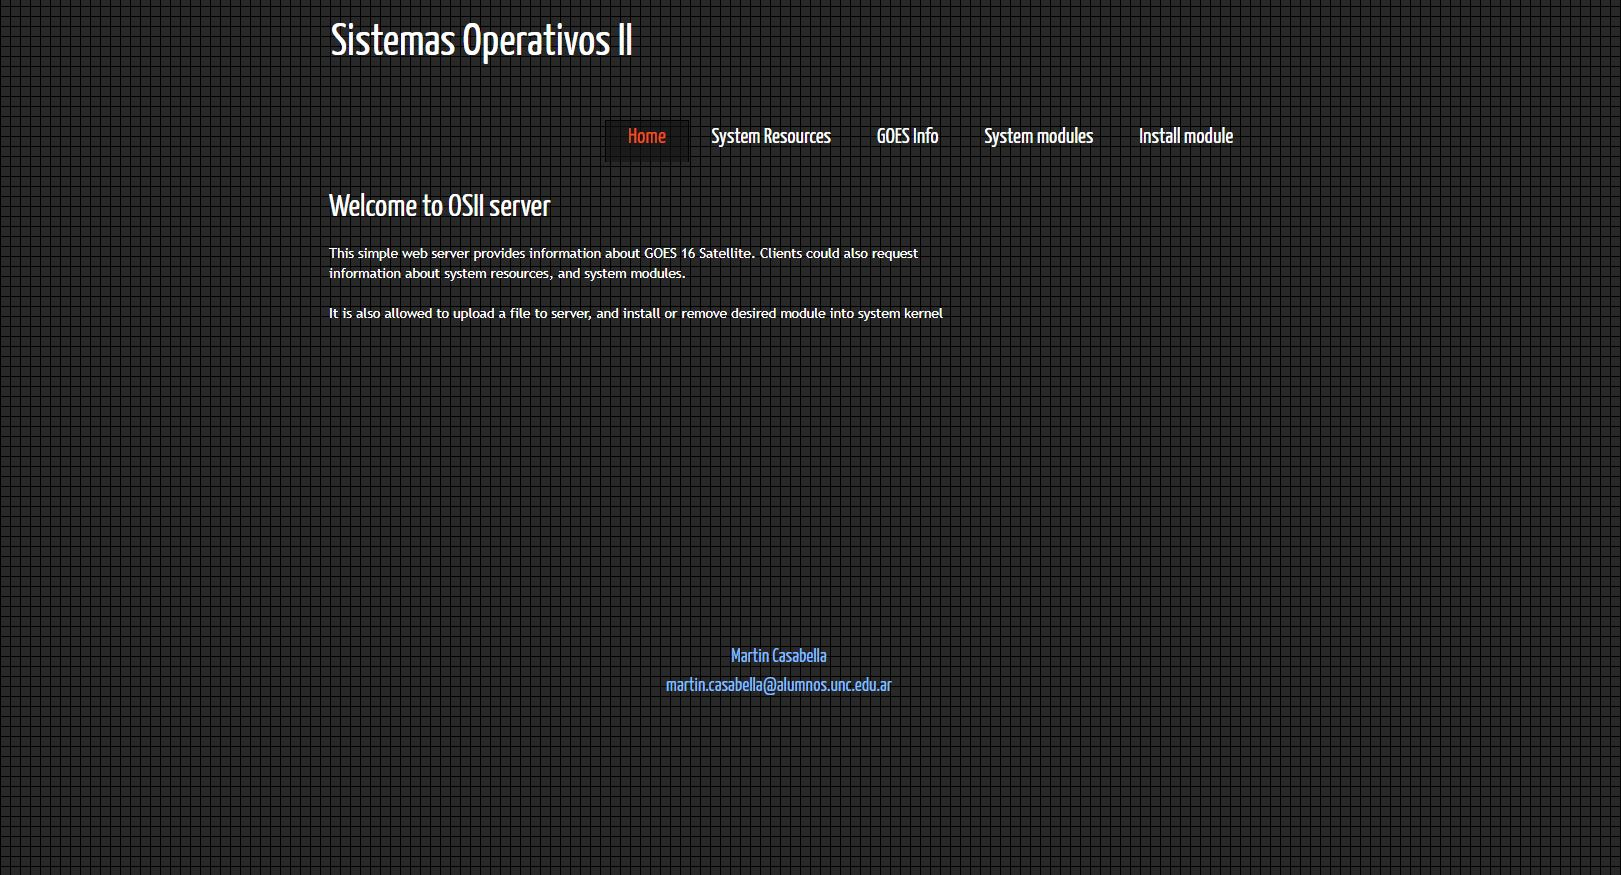
\includegraphics[width=0.8\textwidth]{figures/1.jpg}
       \centering
       \caption{\textbf{\textcolor{Orange}{Pagina principal}}}
    \end{figure}

\begin{figure}[H]
    \centering
      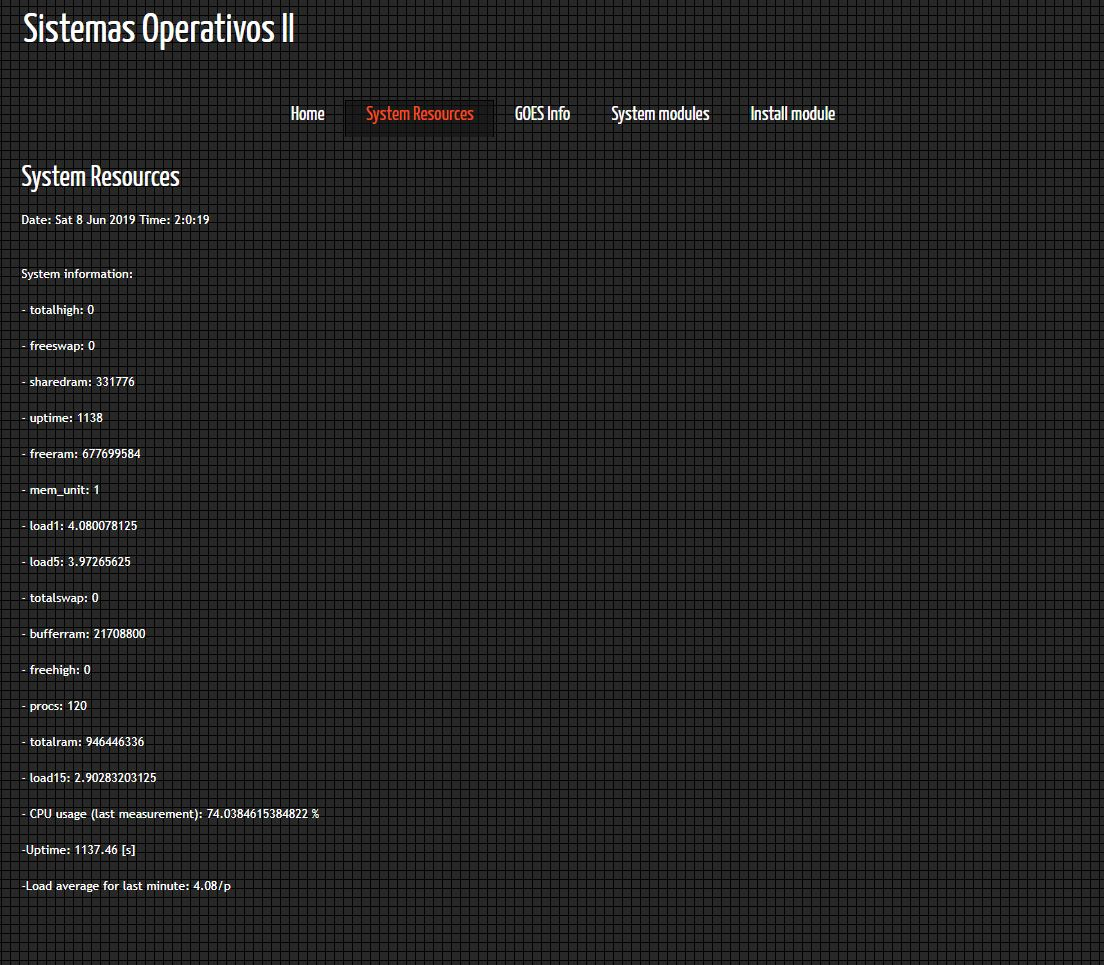
\includegraphics[width=0.8\textwidth]{figures/2.jpg}
       \centering
       \caption{\textbf{\textcolor{Orange}{Pestaña que lista recursos del sistema}}}
    \end{figure}

\begin{figure}[H]
    \centering
      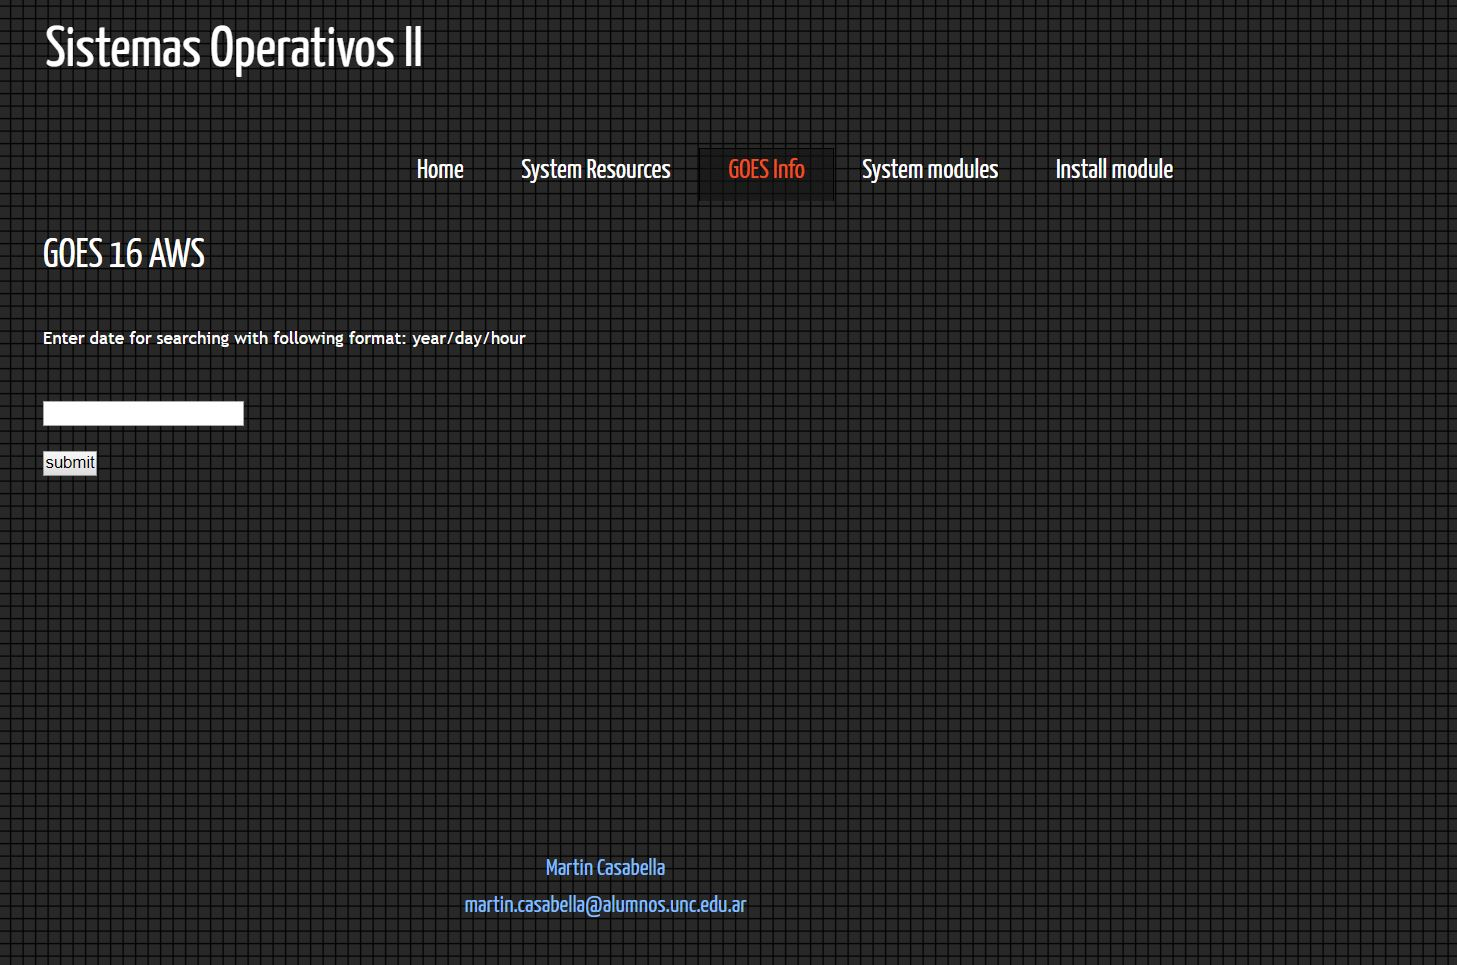
\includegraphics[width=0.8\textwidth]{figures/3.jpg}
       \centering
       \caption{\textbf{\textcolor{Orange}{Pestaña para obtener información del GOES}}}
    \end{figure}

\begin{figure}[H]
    \centering
      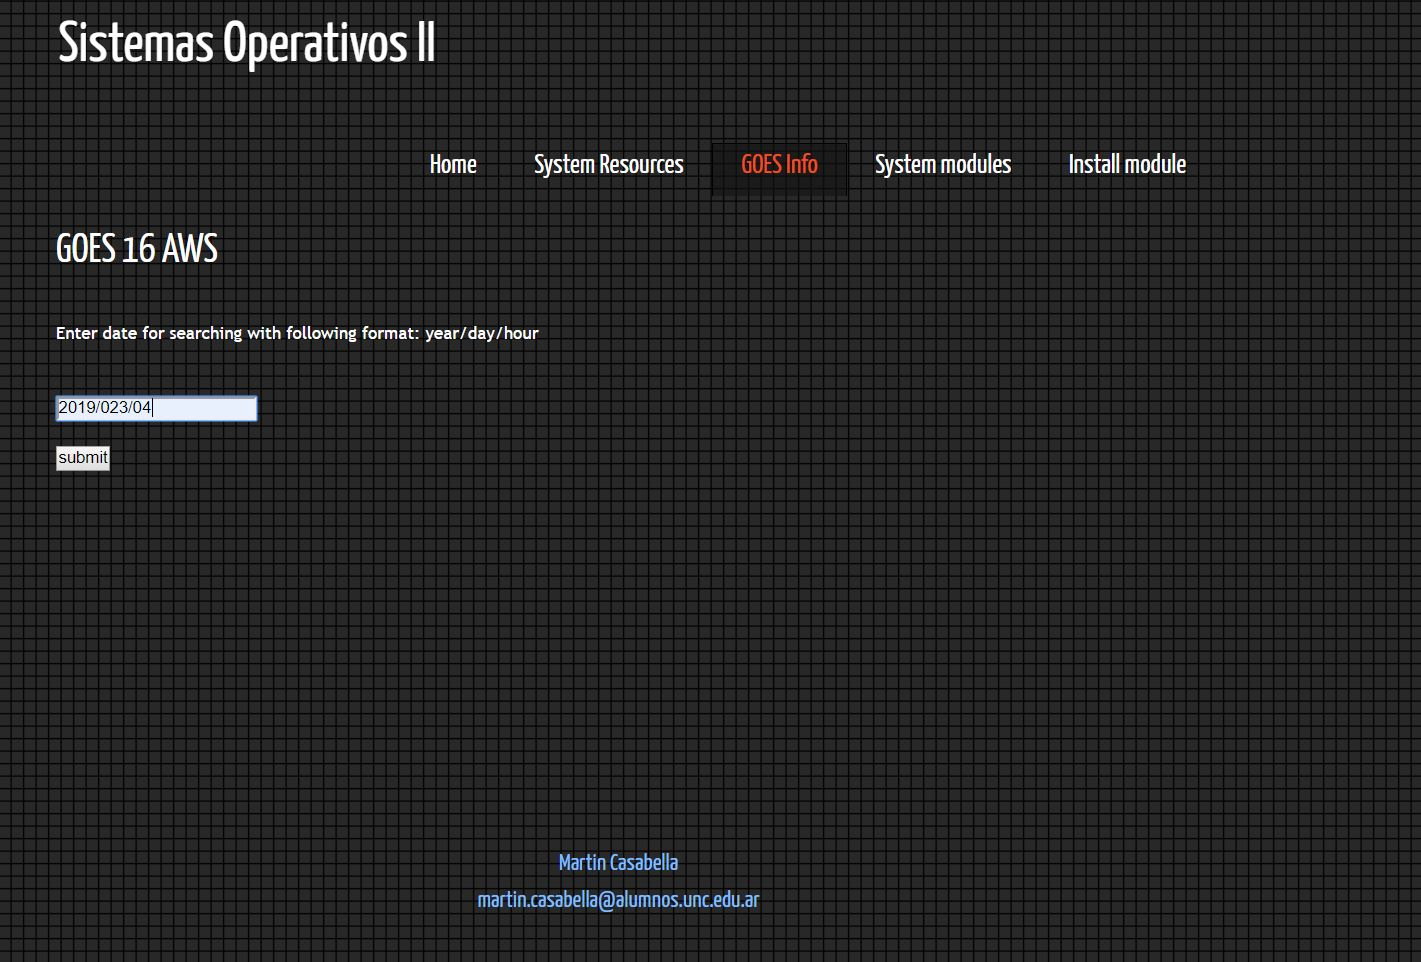
\includegraphics[width=0.8\textwidth]{figures/3bis.jpg}
       \centering
       \caption{\textbf{\textcolor{Orange}{Entrada para testeo}}}       
    \end{figure}

\begin{figure}[H]
    \centering
      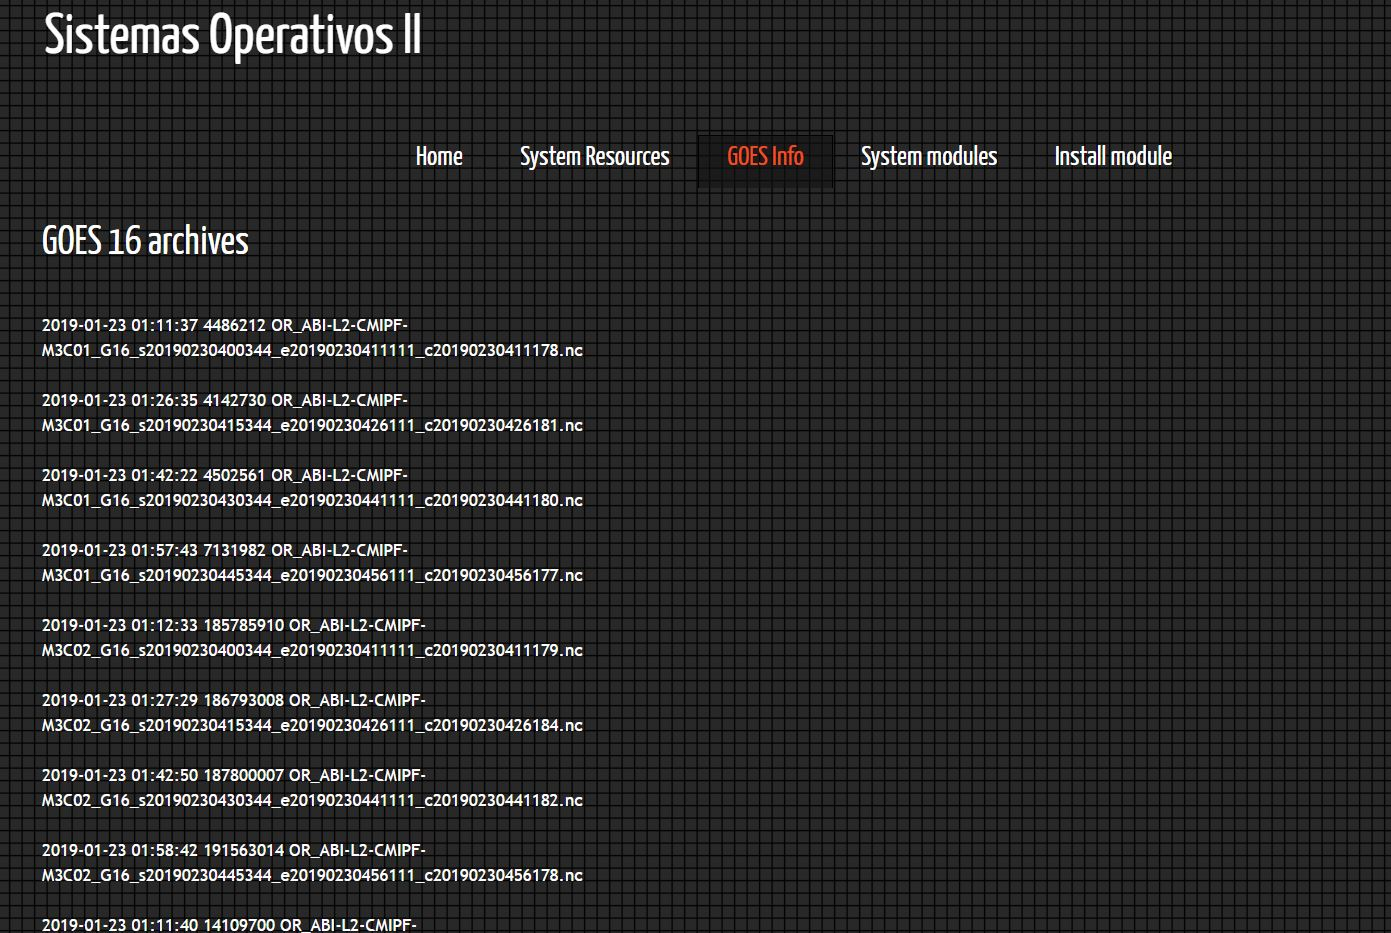
\includegraphics[width=0.8\textwidth]{figures/3bisbis.jpg}
       \centering
       \caption{\textbf{\textcolor{Orange}{Devolución}}}       
    \end{figure}


\begin{figure}[H]
    \centering
      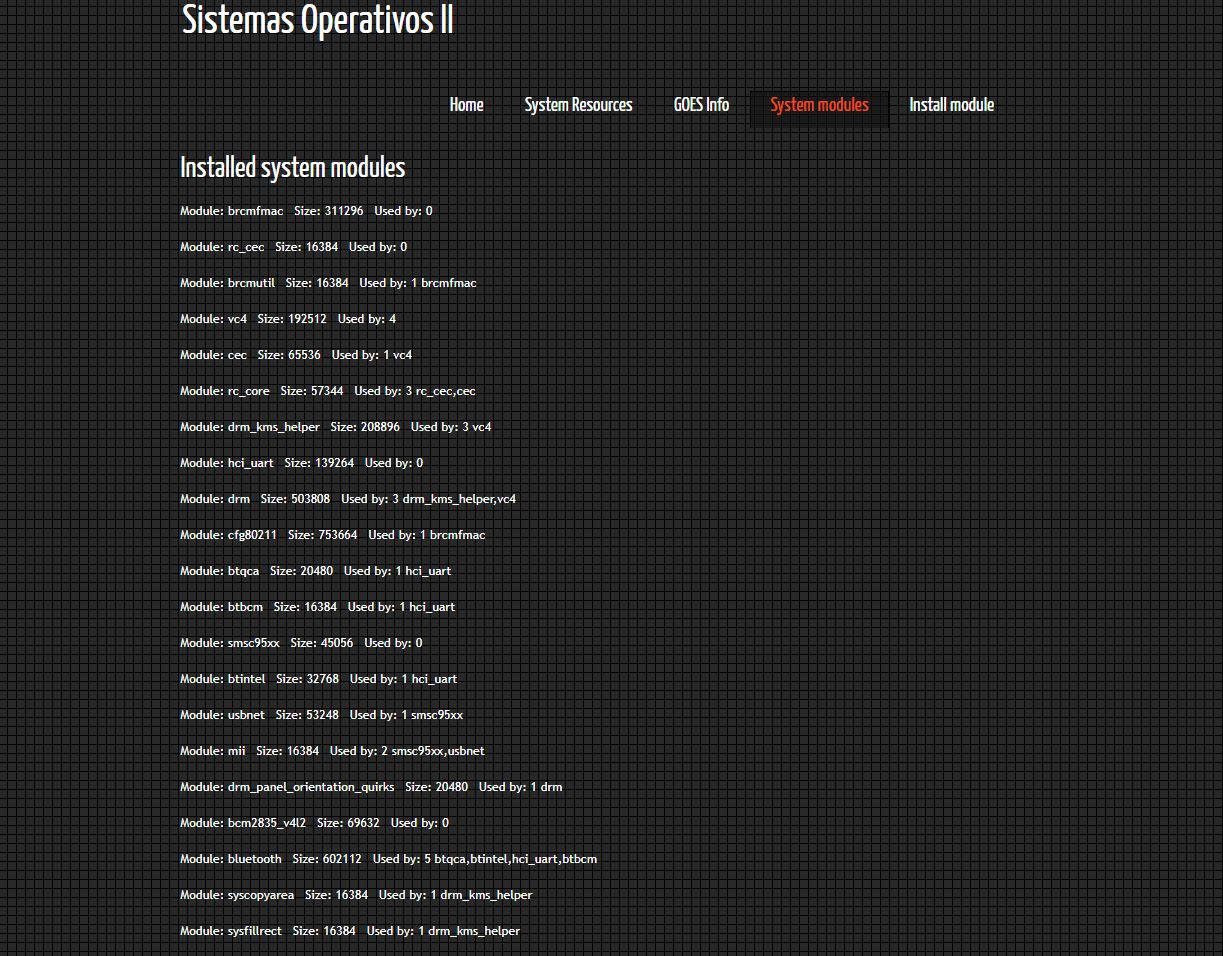
\includegraphics[width=0.7\textwidth]{figures/5.jpg}
       \centering
       \caption{\textbf{\textcolor{Orange}{Pestaña que lista modulos del kernel instalados}}}
    \end{figure}

\begin{figure}[H]
    \centering
      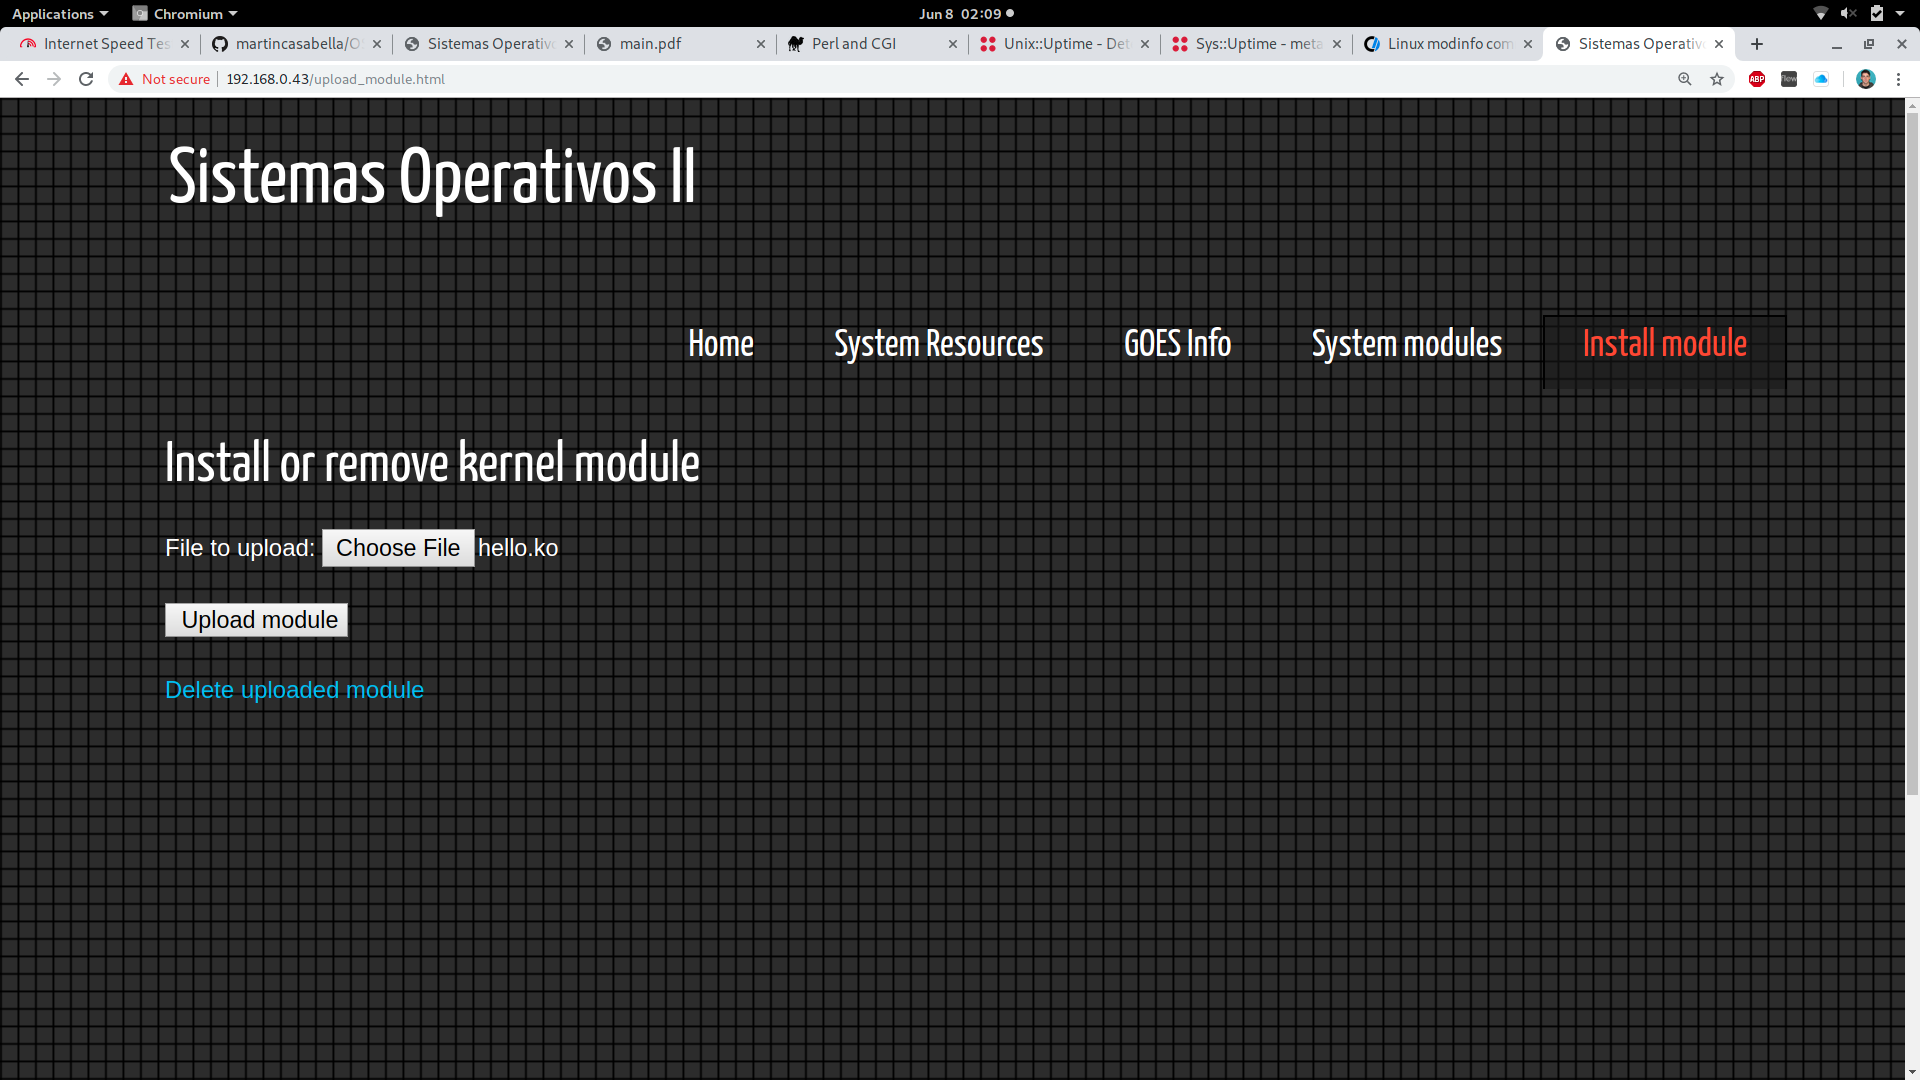
\includegraphics[width=1.0\textwidth]{figures/11.png}
       \centering
\caption{\textbf{\textcolor{Orange}{Pestaña que permite elegir archivo a cargar}}}
         \end{figure}


\begin{figure}[H]
    \centering
      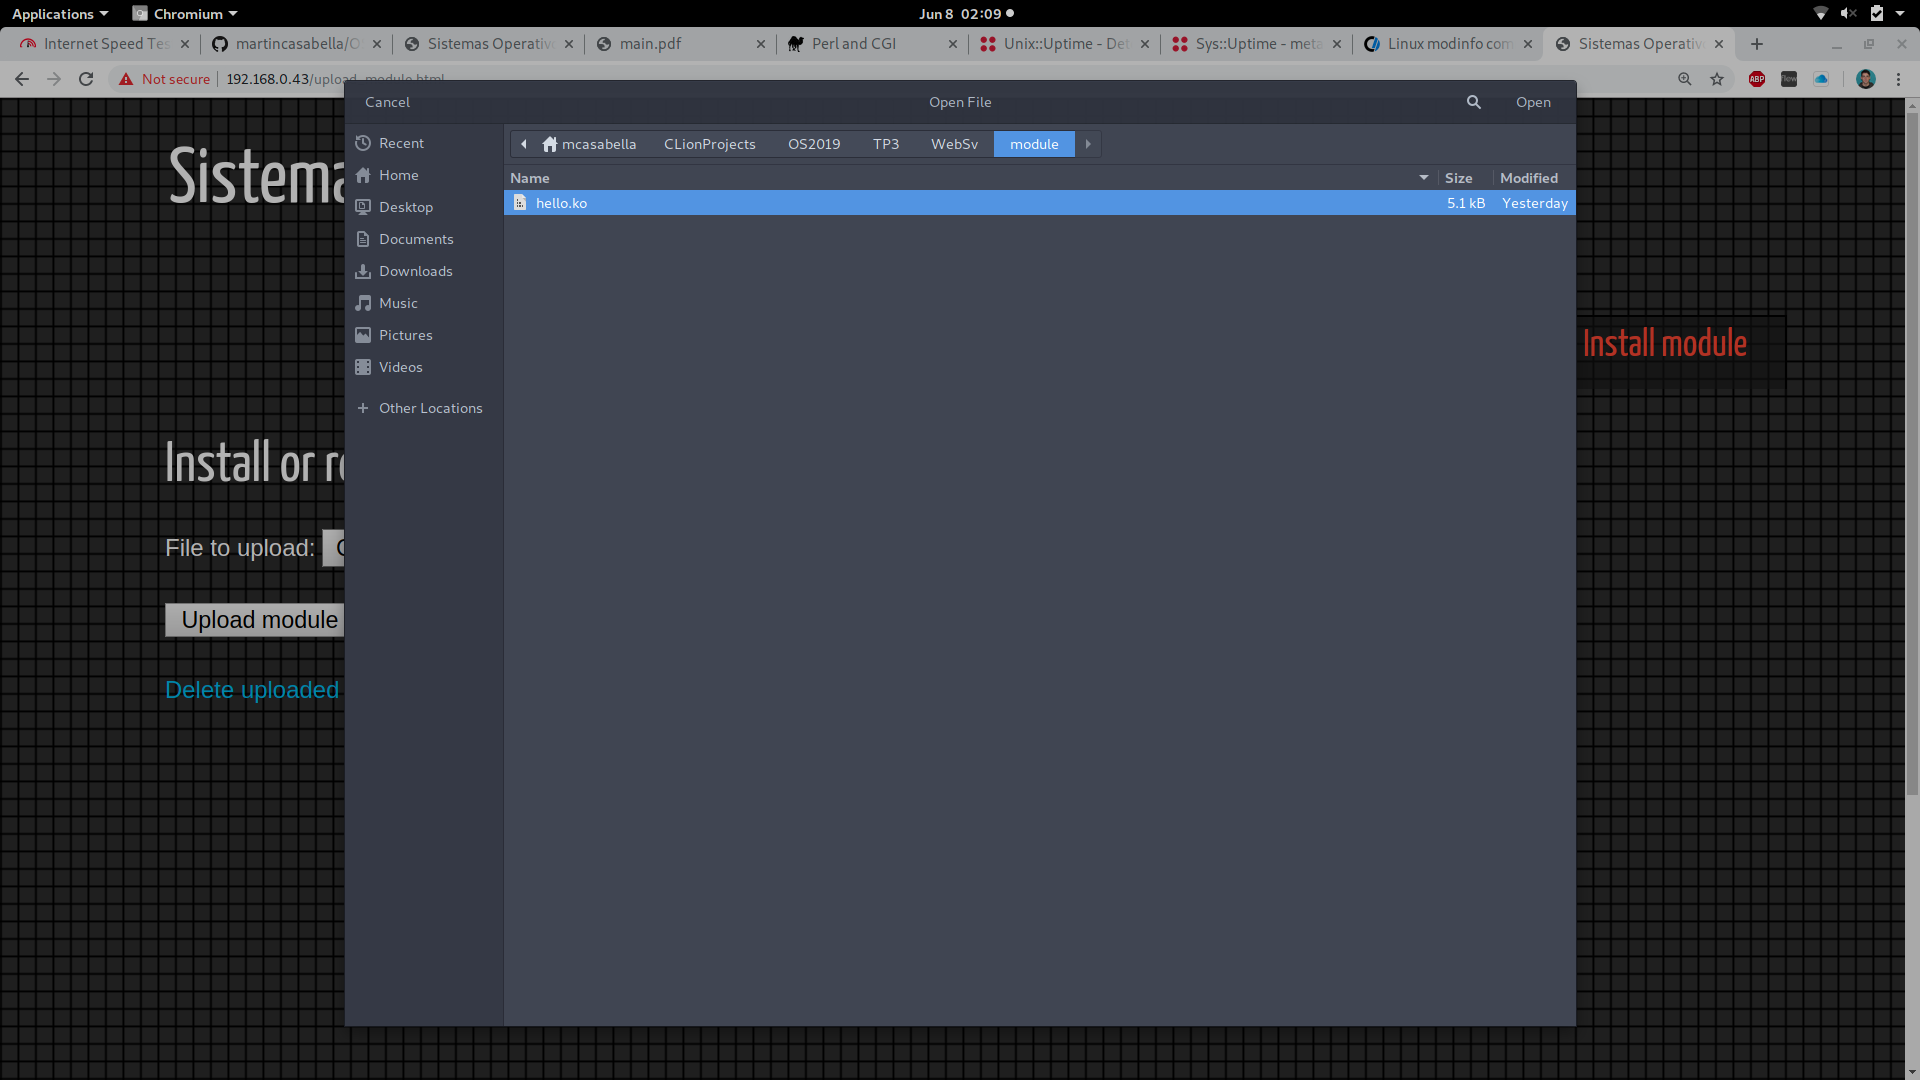
\includegraphics[width=1.0\textwidth]{figures/10.png}
       \centering
       \caption{\textbf{\textcolor{Orange}{Habiendo compilado el modulo, probamos enviarlo al servidor e instalarlo}}}
    \end{figure}




\begin{figure}[H]
    \centering
      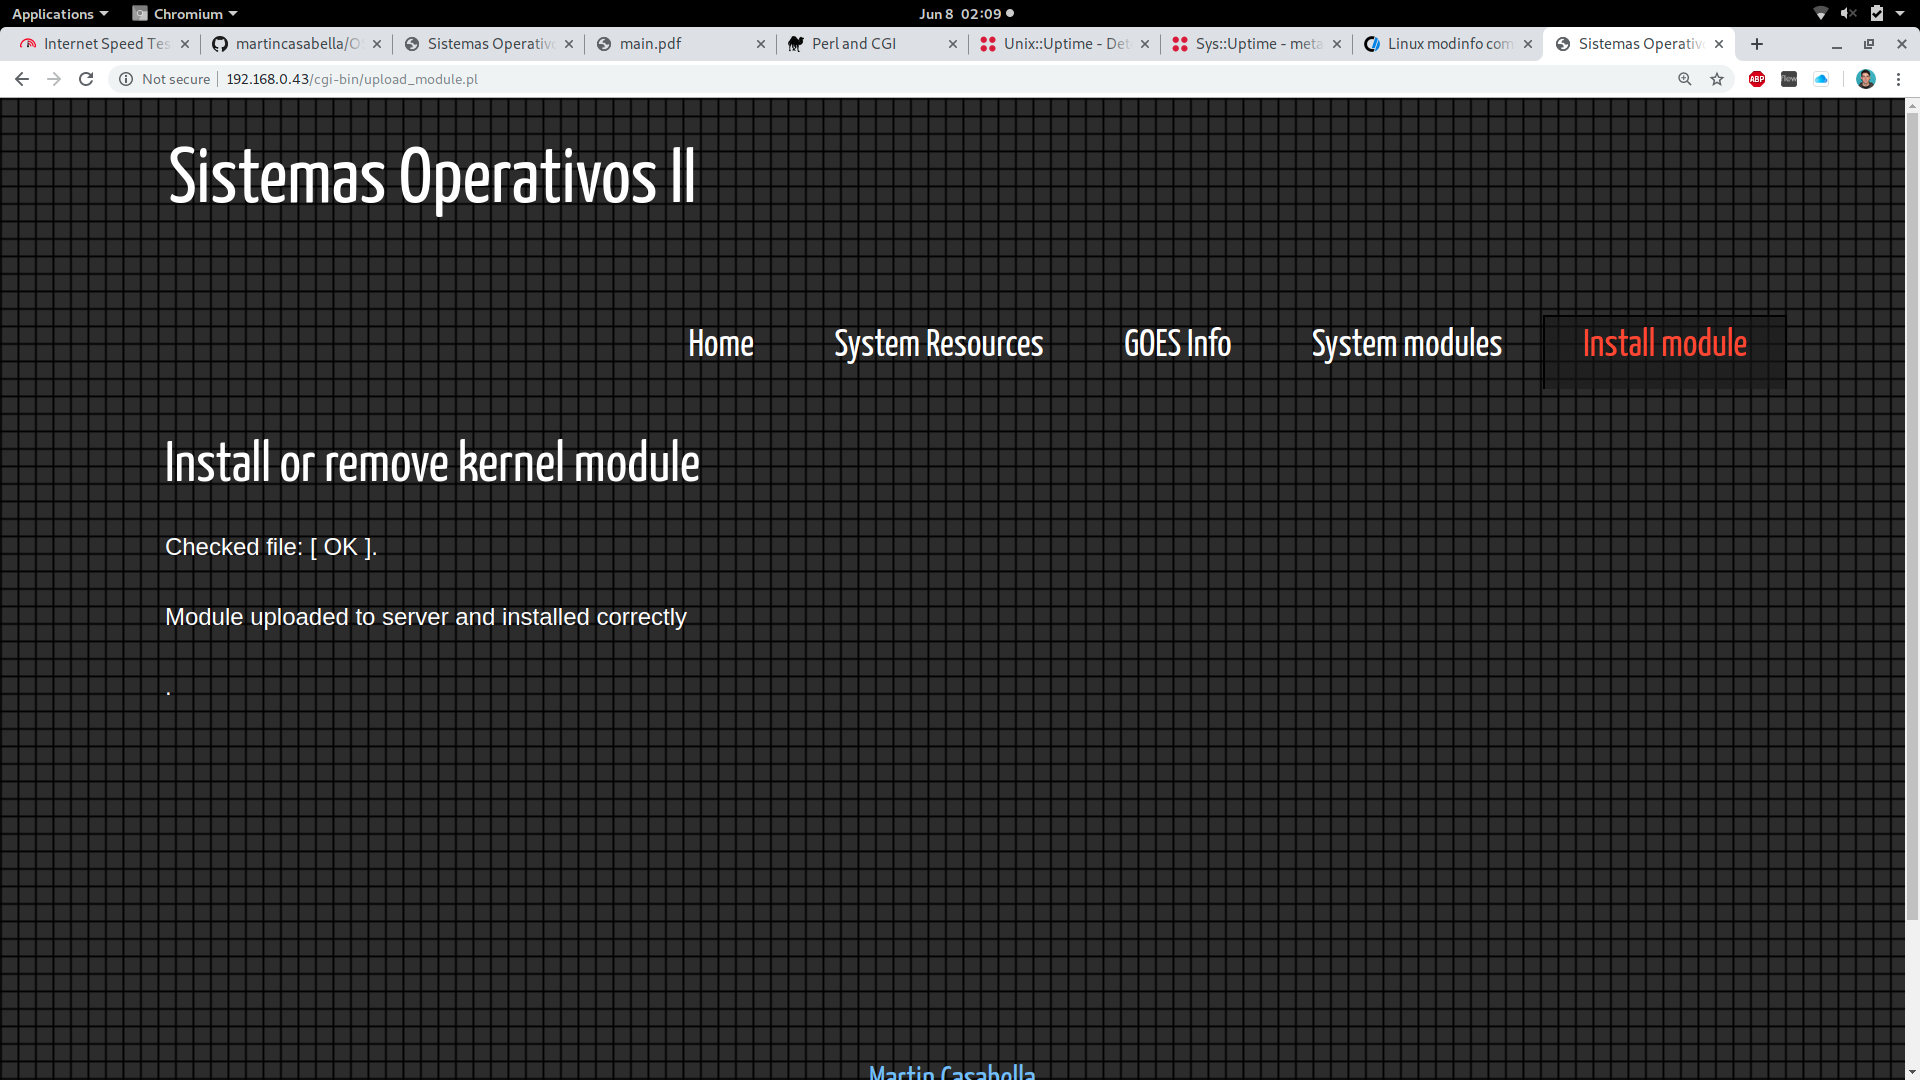
\includegraphics[width=1.0\textwidth]{figures/13.png}
       \centering
       \caption{\textbf{\textcolor{Orange}{Vemos como responde el server ante la carga}}}
         \end{figure}


\begin{figure}[H]
    \centering
      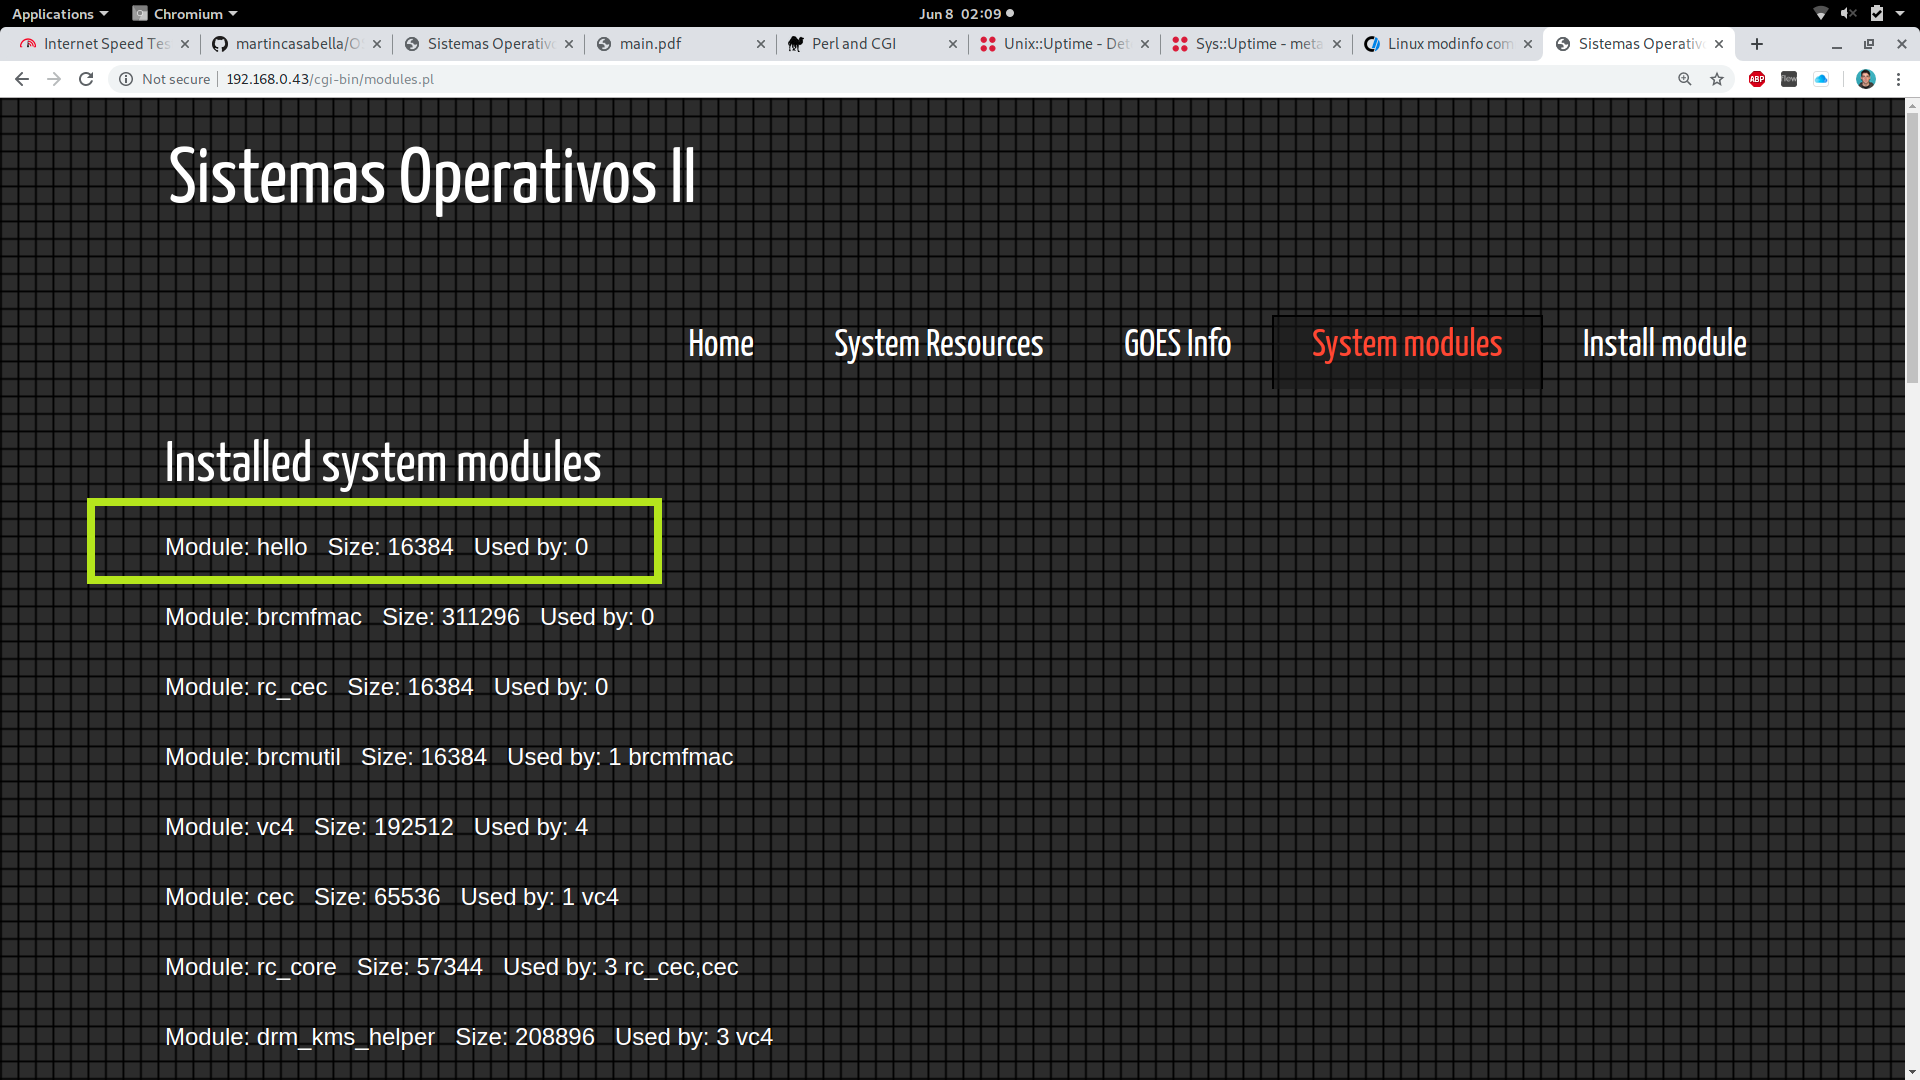
\includegraphics[width=1.0\textwidth]{figures/14.png}
       \centering
       \caption{\textbf{\textcolor{Orange}{Ahora vemos el nuevo modulo listado al volver a pedir la lista de modulos}}}
         \end{figure}
         
         \begin{figure}[H]
    \centering
      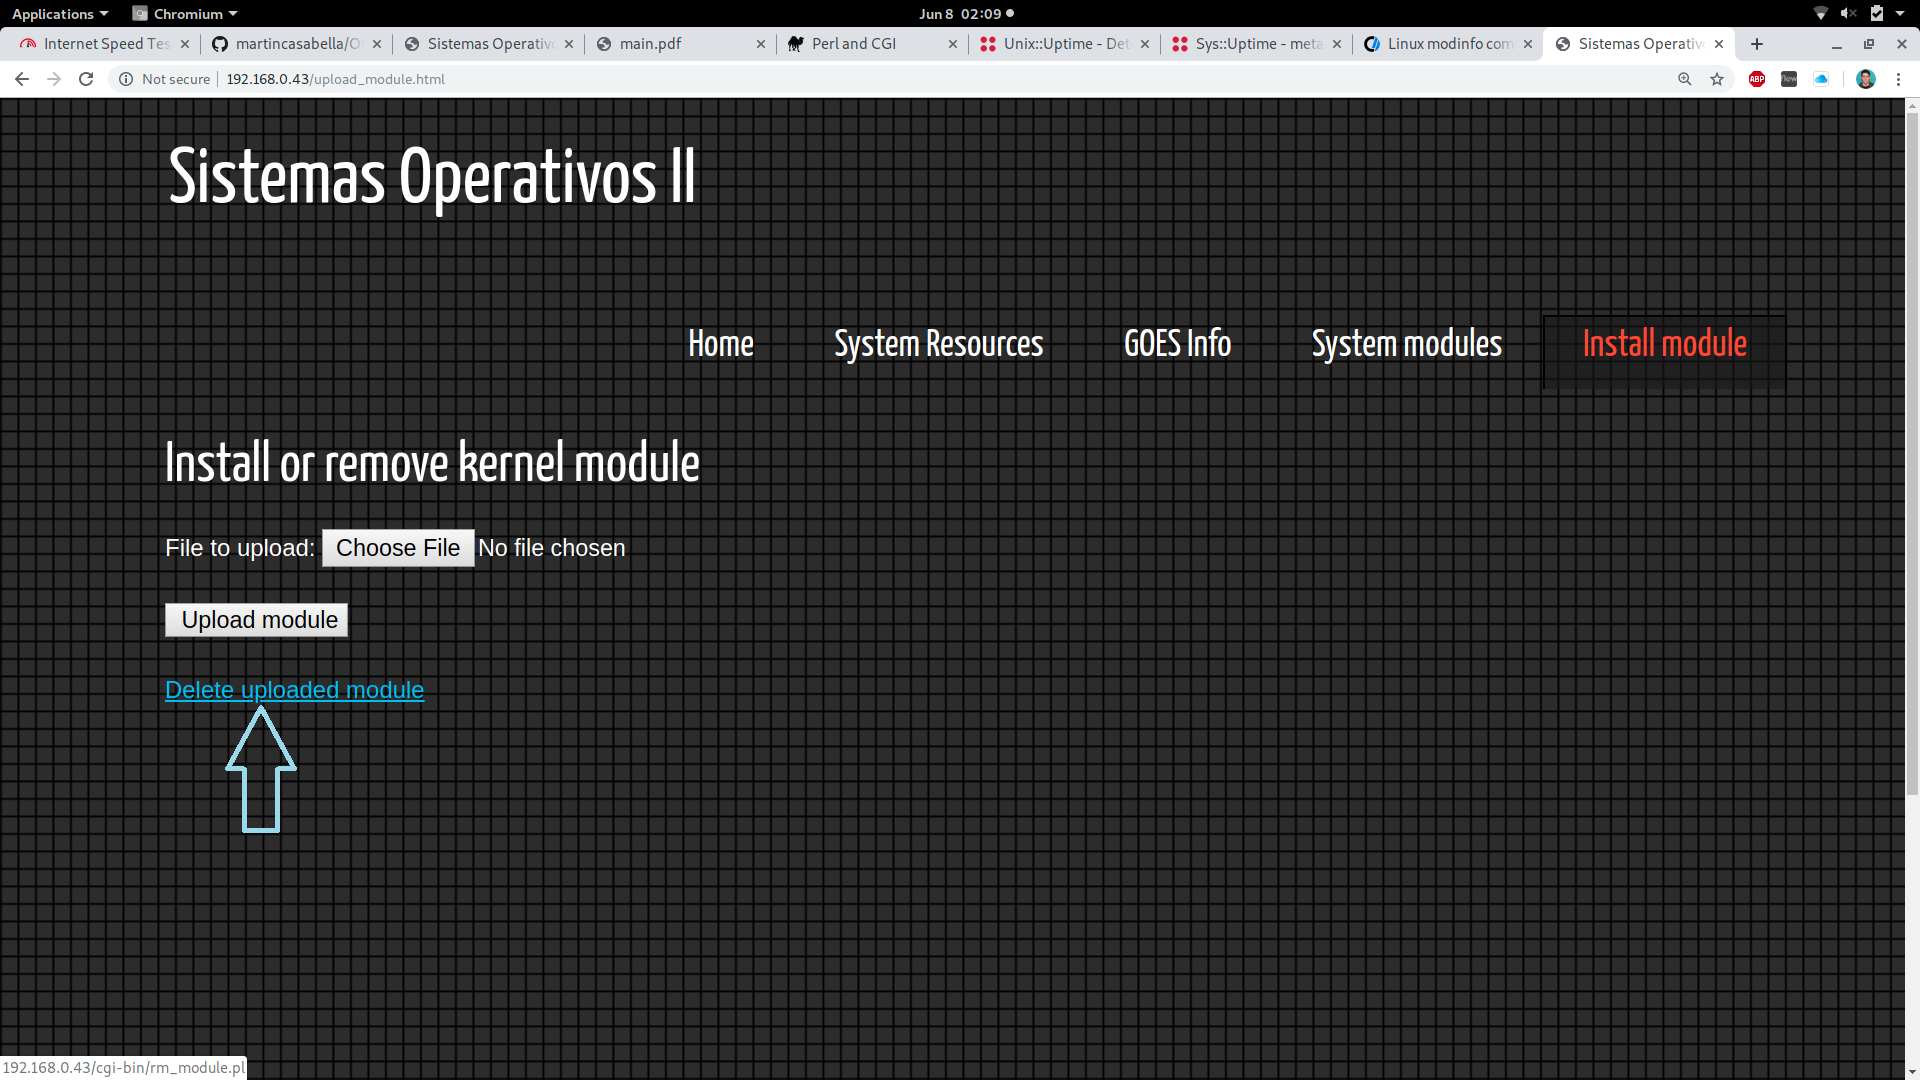
\includegraphics[width=1.0\textwidth]{figures/15.png}
       \centering
       \caption{\textbf{\textcolor{Orange}{Procedemos a querer borrar el modulo}}}
         \end{figure}
         
                  \begin{figure}[H]
    \centering
      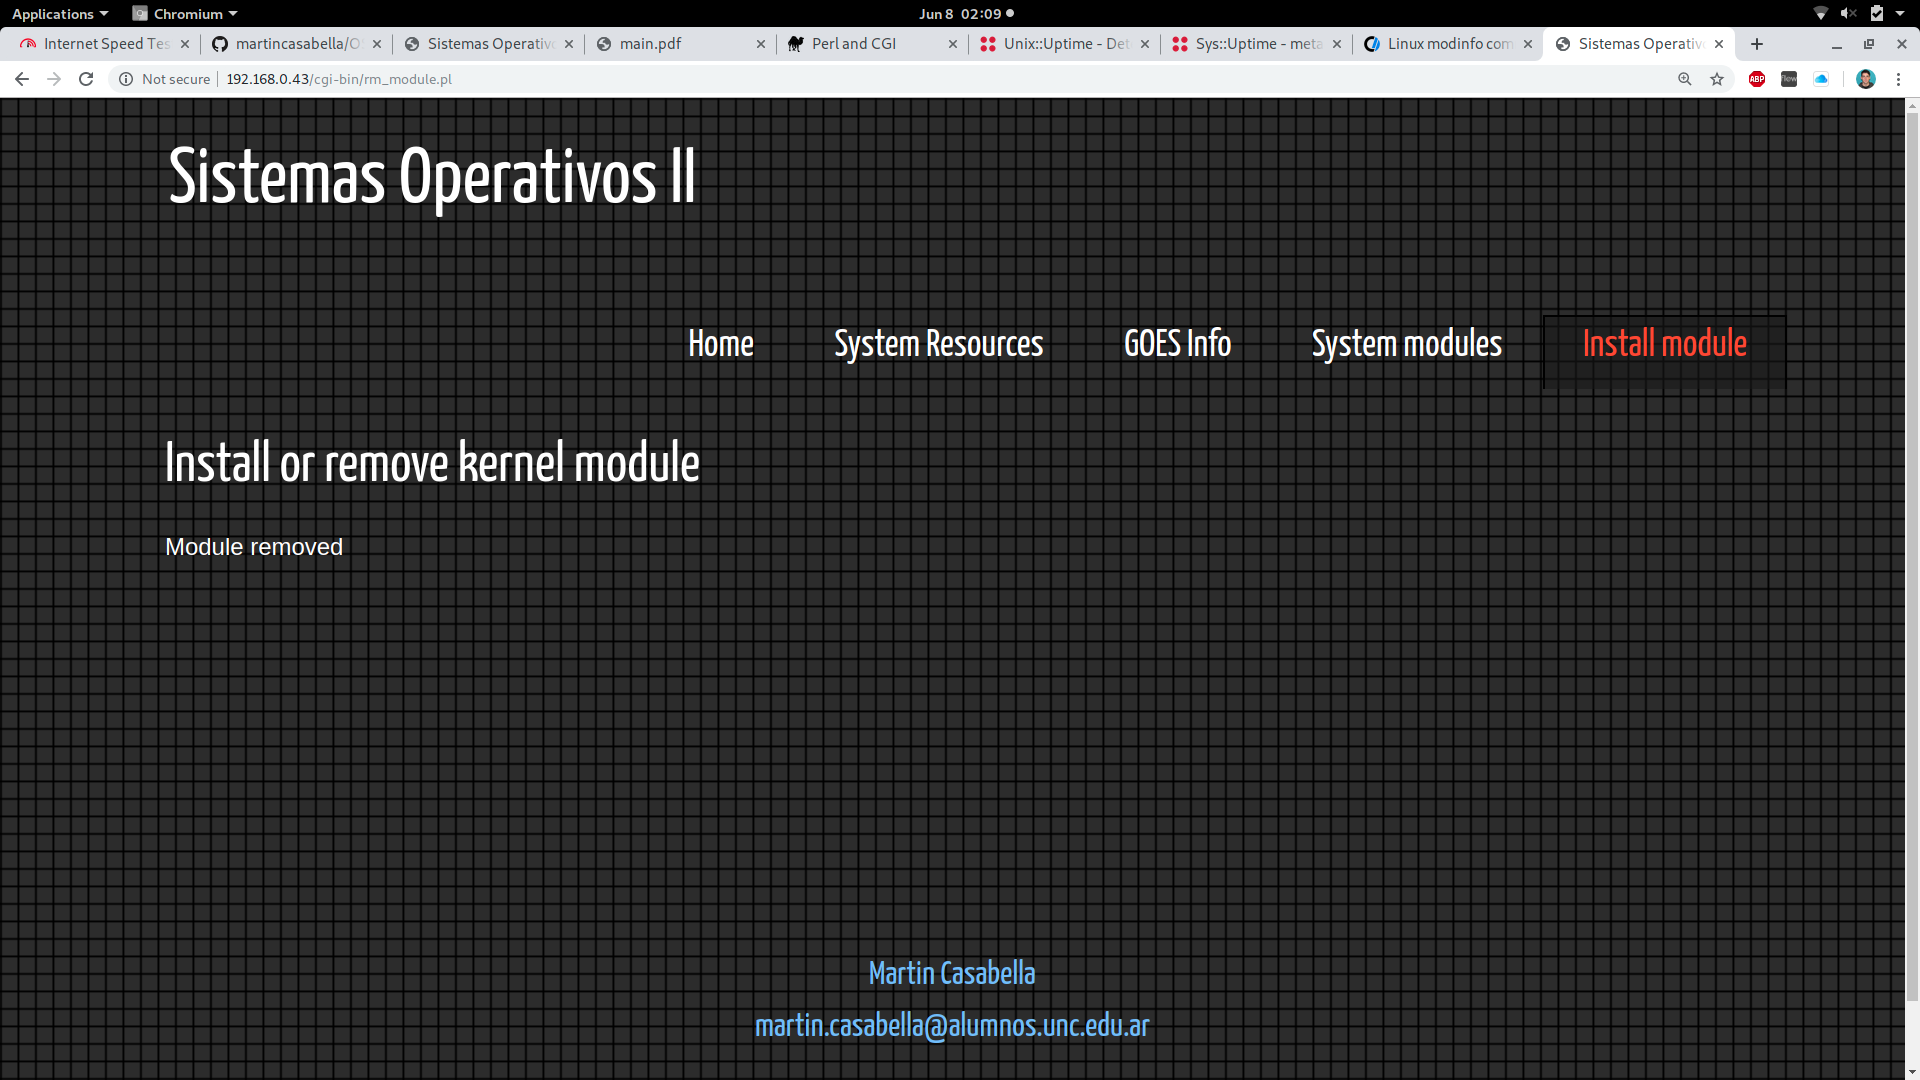
\includegraphics[width=1.0\textwidth]{figures/16.png}
       \centering
       \caption{\textbf{\textcolor{Orange}{Obtenemos respuesta a dicha petición}}}
         \end{figure}
         
                  \begin{figure}[H]
    \centering
      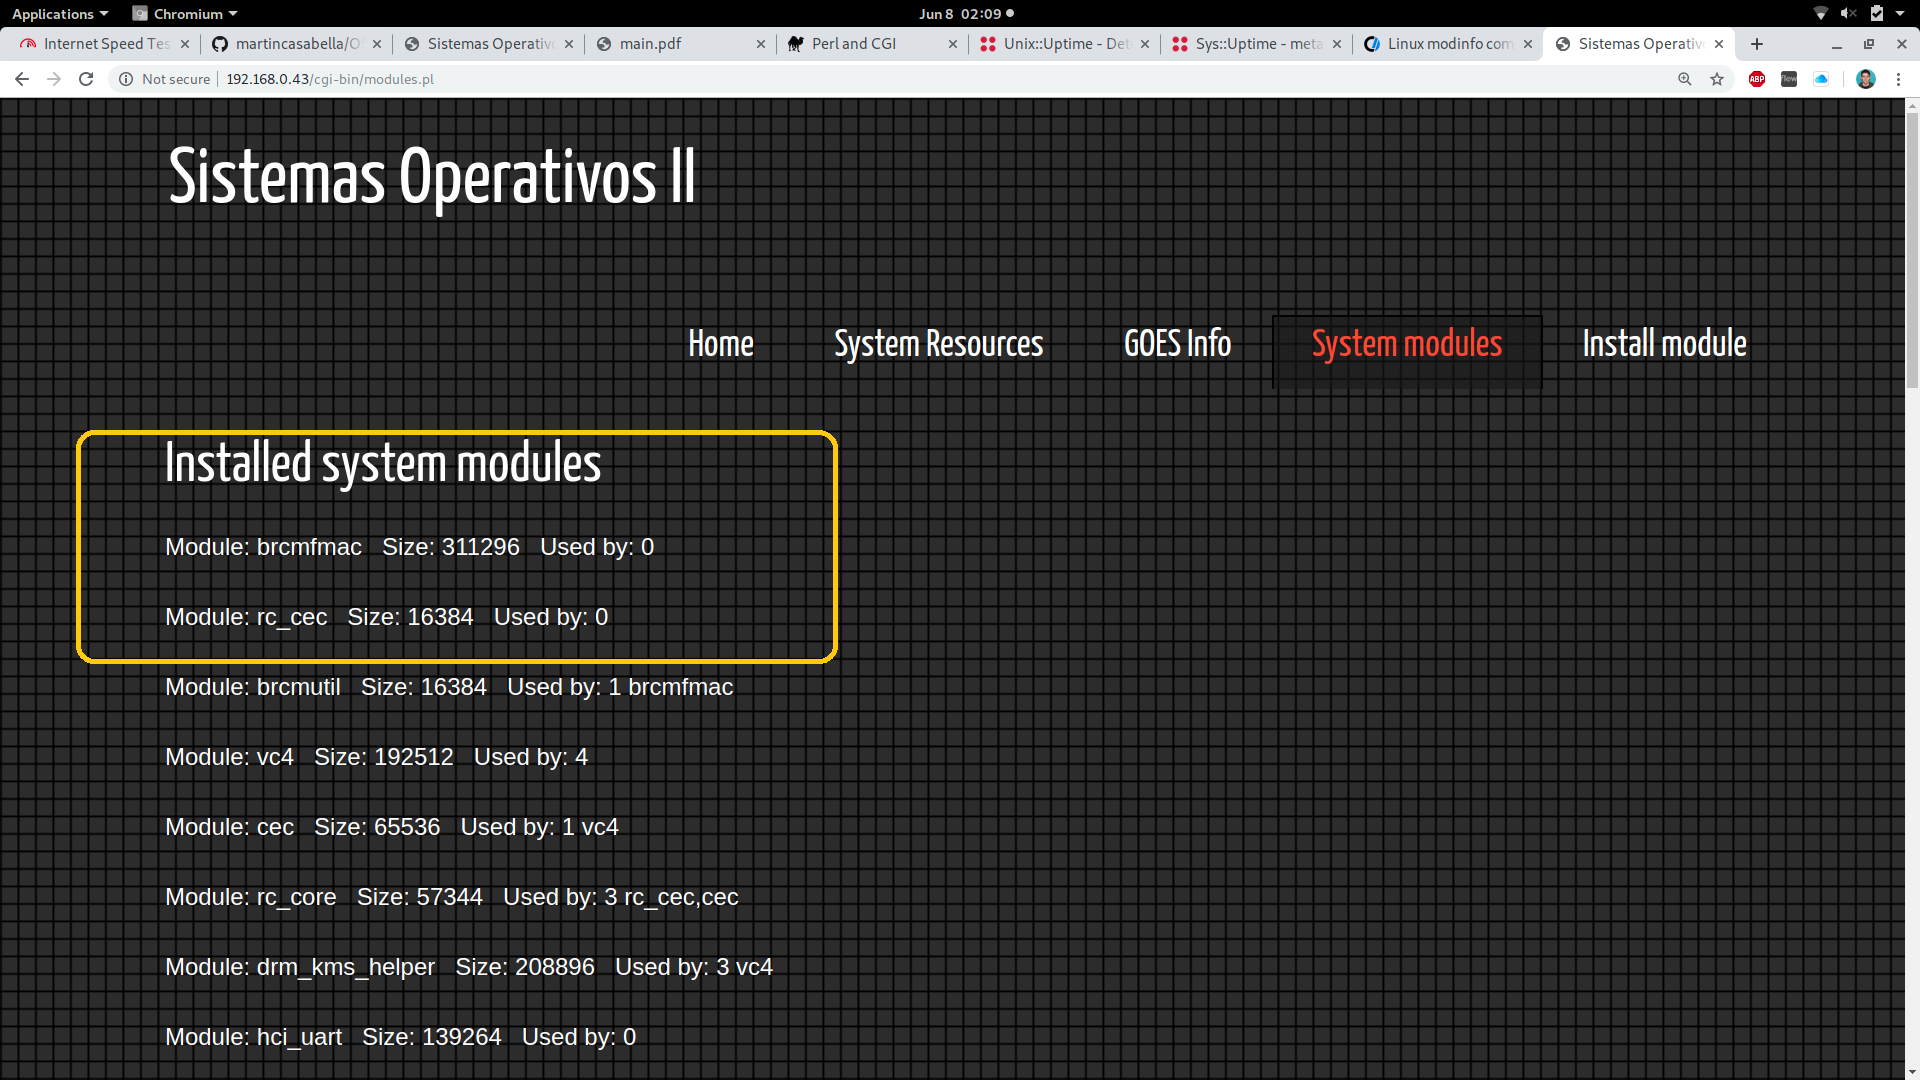
\includegraphics[width=1.0\textwidth]{figures/17.png}
       \centering
       \caption{\textbf{\textcolor{Orange}{Vemos que el modulo fue removido exitosamente}}}
         \end{figure}
         
\clearpage

\section{ Configuración de permisos}


El servidor web debe ser capas de levantar y remover módulos del kernel, para esto hay que darle permisos para que utilice los comandos insmod, modprobe e insmod, aunque
en verdad todos los comandos son los mismo ya que hace un enlace simbólico a Kmod.\\

Se procede a editar el archivo \textbf{sudoers} que contiene los permisos a comandos de los usuarios.\\

\begin{lstlisting}[style=PerlStyle]
#ALIAS para los comandos
Cmnd_Alias MANAGEMOD = /usr/ bin / insmod , /usr/ bin / kmod , /usr/ bin / rmmod
# Al usuario http le permitimos desde todos los hosts (ALL), que ejecute comandos como
# root (root), sin solicitar password (NOPASSWD), los comandos definidos en el alias
# MANAGEMOD
http ALL =( root ) NOPASSWD : MANAGEMOD
\end{lstlisting}



\end{document}